% ==============================================================================
% BÁO CÁO DỰ ÁN - HỌC PHẦN HỌC MÁY (MACHINE LEARNING)
% Đề tài: Dự báo điện năng tiêu thụ của hộ gia đình dựa trên dữ liệu đo theo thời gian
% Trường ĐH Công nghệ Thông tin và Truyền thông
% Biên dịch: xelatex -> biber -> xelatex -> xelatex   (hoặc: .\build.ps1)
%
% Báo cáo phát triển theo các mốc của học phần:
%   Chương 2 - Bài kiểm tra 1 (Tuần 4), Chương 3 - Bài kiểm tra 2 (Tuần 6).
%   Chương 4 (tối ưu hóa và cải tiến, Tuần 8) sẽ được bổ sung khi hoàn thành.
% ==============================================================================
\documentclass{ictureport}

% ==============================================================================
% THÔNG TIN BÁO CÁO (dùng cho trang bìa và PDF)
% ==============================================================================

% Tên đề tài đúng như đã đăng ký với giảng viên (ngắt dòng cho trang bìa)
\newcommand{\coverTitle}{DỰ BÁO ĐIỆN NĂNG TIÊU THỤ CỦA HỘ GIA ĐÌNH\\DỰA TRÊN DỮ LIỆU ĐO THEO THỜI GIAN}
\newcommand{\projectTitle}{Dự báo điện năng tiêu thụ của hộ gia đình dựa trên dữ liệu đo theo thời gian}

% Nhóm và giảng viên. Để trống \groupName thì trang bìa không in dòng "Tên nhóm".
\newcommand{\groupName}{}
\newcommand{\memberOne}{Trần Trọng Hoàn \#}
\newcommand{\memberTwo}{Vũ Ngọc Quý}
\newcommand{\className}{KHMT K22A}
\newcommand{\instructorName}{TS. Nguyễn Tuấn Anh}

\newcommand{\reportYear}{2026}
\newcommand{\logoPath}{figures/logo_ictu.png}

% ==============================================================================
% CẤU HÌNH BỔ SUNG: tài liệu tham khảo, liên kết, macro của đề tài
% ==============================================================================

% Tài liệu tham khảo dạng [n] (IEEE) qua BibLaTeX/Biber
\usepackage[
    backend=biber,
    style=ieee,
    sorting=none,
    doi=true,
    isbn=false,
    url=true
]{biblatex}
\addbibresource{references.bib}
\setlength{\bibitemsep}{3pt}

% Liên kết nội bộ (không tô màu, giống bản in Word)
\usepackage{hyperref}
\hypersetup{
    hidelinks,
    pdfauthor={Trần Trọng Hoàn, Vũ Ngọc Quý},
    pdftitle={\projectTitle},
    pdfsubject={Báo cáo dự án học phần Học máy},
    pdfkeywords={Học máy, dự báo chuỗi thời gian, điện năng, Random Forest, XGBoost}
}

% Macro tiện ích
\DeclareRobustCommand{\code}[1]{\texttt{\detokenize{#1}}}
\usepackage{float}
\usepackage{bm}
\DeclareMathOperator*{\argmin}{arg\,min}
\usepackage{xurl}
\setcounter{biburlnumpenalty}{100}
\setcounter{biburllcpenalty}{100}
\setcounter{biburlucpenalty}{100}


\begin{document}

% ------------------------------------------------------------------------------
% 1. TRANG BÌA (không đánh số trang)
% ------------------------------------------------------------------------------
\makecoverpage

% ------------------------------------------------------------------------------
% 2. PHẦN ĐẦU (đánh số trang La Mã)
% ------------------------------------------------------------------------------
\pagenumbering{roman}
\setcounter{page}{1}

\unnumberedchapter{LỜI CẢM ƠN}

% Lời cảm ơn là lời của nhóm: nhóm có thể sửa lại bằng lời văn của mình.
Chúng em xin chân thành cảm ơn TS. Nguyễn Tuấn Anh đã hướng dẫn, góp ý và định hướng cho nhóm trong suốt quá trình thực hiện dự án học phần Học máy.

Chúng em cũng cảm ơn các tác giả G.~Hébrail và A.~Bérard cùng Kho dữ liệu Học máy UCI đã công bố bộ dữ liệu được sử dụng trong đề tài.

Do kiến thức và thời gian còn hạn chế, báo cáo khó tránh khỏi thiếu sót. Chúng em rất mong nhận được góp ý của thầy để hoàn thiện dự án ở các giai đoạn tiếp theo.

\vspace{1cm}
\begin{flushright}
\begin{tabular}{c}
Thái Nguyên, tháng 11 năm 2026\\
Nhóm sinh viên thực hiện\\[1.8cm]
Trần Trọng Hoàn \# \qquad Vũ Ngọc Quý
\end{tabular}
\end{flushright}

\tableofcontents
\unnumberedchapter{PHÂN CÔNG NHIỆM VỤ}

% Nhóm kiểm tra lại cho đúng thực tế; mỗi thành viên commit phần việc của mình lên Git.
\noindent\textbf{Phân công nhiệm vụ theo tiến độ thực hiện:}

\begingroup
\setstretch{1.15}
\noindent
\begin{tabularx}{\textwidth}{|>{\centering\arraybackslash}p{1.0cm}|>{\raggedright\arraybackslash}X|>{\raggedright\arraybackslash}p{4.2cm}|}
\hline
\textbf{Stt} & \centering\arraybackslash\textbf{Tên nhiệm vụ} & \centering\arraybackslash\textbf{Người thực hiện} \\ \hline
1 & Chọn đề tài và bộ dữ liệu, phát biểu bài toán, xác định chỉ số đánh giá (tuần 1--3) & Cả nhóm \\ \hline
2 & Nạp dữ liệu, từ điển dữ liệu, thống kê mô tả, phân bố các biến (tuần 3--4) & Trần Trọng Hoàn \\ \hline
3 & Xây dựng nhãn theo giờ, tương quan, tự tương quan, phân tích theo ngày (tuần 3--4) & Vũ Ngọc Quý \\ \hline
4 & Định lượng và xử lý vấn đề chất lượng dữ liệu, so sánh trước -- sau (tuần 3--4) & Trần Trọng Hoàn \\ \hline
5 & Bảng có giám sát, chia dữ liệu theo thời gian, pipeline tiền xử lý (tuần 4) & Vũ Ngọc Quý \\ \hline
6 & Thiết kế đặc trưng, cài đặt mô hình cơ sở và mô hình học máy, kiểm định chéo (tuần 5--6) & Trần Trọng Hoàn \\ \hline
7 & Phân tích lỗi, so sánh huấn luyện -- kiểm định, tầm quan trọng đặc trưng (tuần 5--6) & Vũ Ngọc Quý \\ \hline
8 & Viết báo cáo, rà soát mã nguồn và kết quả (tuần 4, 6) & Cả nhóm \\ \hline
\end{tabularx}
\endgroup

\vspace{0.6cm}
\noindent\textbf{Phân công nhiệm vụ theo thành viên thực hiện:}

\begingroup
\setstretch{1.15}
\noindent
\begin{tabularx}{\textwidth}{|>{\centering\arraybackslash}p{1.0cm}|>{\raggedright\arraybackslash}p{3.6cm}|>{\raggedright\arraybackslash}X|>{\centering\arraybackslash}p{2.2cm}|}
\hline
\textbf{Stt} & \centering\arraybackslash\textbf{Thành viên} & \centering\arraybackslash\textbf{Nhiệm vụ} & \textbf{Chữ ký} \\ \hline
1 & Trần Trọng Hoàn \# & - Nhóm trưởng; quản lý tiến độ và kho mã nguồn.\newline - Dữ liệu: nạp dữ liệu, thống kê mô tả, chất lượng dữ liệu.\newline - Mô hình: thiết kế đặc trưng, cài đặt mô hình, kiểm định chéo. & \\[1.2cm] \hline
2 & Vũ Ngọc Quý & - Nhãn theo giờ, tương quan và tính mùa vụ.\newline - Chuẩn bị dữ liệu: chia theo thời gian, pipeline tiền xử lý.\newline - Phân tích lỗi và tầm quan trọng đặc trưng. & \\[1.2cm] \hline
\end{tabularx}
\endgroup

\listoftables
\listoffigures
\unnumberedchapter{DANH MỤC CÁC TỪ VIẾT TẮT}

\begingroup
\setstretch{1.0}
\renewcommand{\arraystretch}{1.3}
\begin{longtable}{|p{3.0cm}|p{11.6cm}|}
    \hline
    \centering\arraybackslash\textbf{Từ viết tắt} & \centering\arraybackslash\textbf{Tên đầy đủ / Diễn giải} \\
    \hline
    \endhead
        ACF & Autocorrelation Function -- hàm tự tương quan \\ \hline
        CART & Classification and Regression Trees \\ \hline
        CV & Cross-Validation -- kiểm định chéo \\ \hline
        EDA & Exploratory Data Analysis -- phân tích khám phá dữ liệu \\ \hline
        GAP & \code{Global_active_power} -- công suất tác dụng toàn hộ \\ \hline
        IQR & Interquartile Range -- khoảng tứ phân vị \\ \hline
        LR & Linear Regression -- hồi quy tuyến tính \\ \hline
        MAE & Mean Absolute Error \\ \hline
        MAPE & Mean Absolute Percentage Error \\ \hline
        MCAR & Missing Completely At Random \\ \hline
        NaN & Not a Number -- giá trị khuyết thiếu \\ \hline
        OLS & Ordinary Least Squares -- bình phương tối thiểu \\ \hline
        RF & Random Forest \\ \hline
        RMSE & Root Mean Squared Error \\ \hline
        SNaive & Seasonal Naive -- mô hình cơ sở lặp lại giá trị cùng mùa \\ \hline
        UCI & UC Irvine Machine Learning Repository \\ \hline
        XGBoost & eXtreme Gradient Boosting \\ \hline
\end{longtable}
\endgroup

\unnumberedchapter{MỞ ĐẦU}
\label{chap:introduction}

Dự báo phụ tải điện là bài toán nền tảng trong vận hành và lập kế hoạch hệ thống điện~\cite{hong2016probabilistic}. Ở cấp độ một hộ gia đình, điện năng tiêu thụ biến động mạnh theo giờ trong ngày, theo ngày trong tuần và theo mùa, vì phụ thuộc trực tiếp vào thói quen sinh hoạt. Biết trước mức tiêu thụ trong vài giờ tới giúp người dùng chủ động sử dụng điện, đồng thời là bài toán phù hợp để thực hành trọn vẹn quy trình học máy: từ phát biểu bài toán, khảo sát và làm sạch dữ liệu đến xây dựng, đánh giá và cải tiến mô hình.

Nhóm lựa chọn đề tài ``Dự báo điện năng tiêu thụ của hộ gia đình dựa trên dữ liệu đo theo thời gian'', sử dụng bộ dữ liệu công khai Individual Household Electric Power Consumption của Kho dữ liệu Học máy UCI~\cite{hebrail2006uci}. Theo định hướng của giảng viên, đề tài gồm bốn nội dung: (1) nghiên cứu bài toán dự báo chuỗi thời gian và cách chuyển về hồi quy có giám sát bằng đặc trưng trễ, cửa sổ trượt và đặc trưng lịch; (2) tiền xử lý dữ liệu, tổng hợp theo giờ và theo ngày, phân tích tính mùa vụ; (3) xây dựng và so sánh các mô hình cơ sở (naive, seasonal naive) với Linear Regression, Random Forest và XGBoost, chia dữ liệu theo thời gian để tránh rò rỉ dữ liệu; (4) đánh giá bằng MAE, RMSE, MAPE theo các tầm dự báo và phân tích sai số theo thời điểm trong ngày.

Báo cáo được xây dựng theo các mốc của học phần và hiện gồm ba chương: Chương~\ref{chap:theory} trình bày cơ sở lý thuyết; Chương~\ref{chap:data} trình bày bài toán, dữ liệu và tiền xử lý (Bài kiểm tra 1); Chương~\ref{chap:models} trình bày việc xây dựng, huấn luyện và đánh giá mô hình (Bài kiểm tra 2). Nội dung tối ưu hóa và cải tiến mô hình sẽ được bổ sung ở giai đoạn tiếp theo.


% ------------------------------------------------------------------------------
% 3. NỘI DUNG CHÍNH (đánh số trang Ả Rập)
% ------------------------------------------------------------------------------
\clearpage
\pagenumbering{arabic}
\setcounter{page}{1}

\chapter{CƠ SỞ LÝ THUYẾT}
\label{chap:theory}

Chương này trình bày các khái niệm nền tảng của học máy, cách tiếp cận bài toán dự báo chuỗi thời gian bằng hồi quy có giám sát, các mô hình được sử dụng trong đề tài và phương pháp đánh giá mô hình.

\section{Tổng quan về học máy}
\label{sec:ml_overview}

\subsection{Trí tuệ nhân tạo và học máy}
Trí tuệ nhân tạo (Artificial Intelligence) là lĩnh vực nghiên cứu và xây dựng các tác tử có khả năng tiếp nhận thông tin từ môi trường và hành động để đạt mục tiêu~\cite{russell2020artificial}. Học máy (Machine Learning) là một nhánh của trí tuệ nhân tạo, nghiên cứu các chương trình tự cải thiện hiệu năng nhờ dữ liệu thay vì được lập trình tường minh từng quy tắc. Theo Mitchell~\cite{mitchell1997machine}, một chương trình được gọi là học từ kinh nghiệm $E$ đối với lớp nhiệm vụ $T$ và thước đo hiệu năng $P$ nếu hiệu năng trên $T$, đo bằng $P$, được cải thiện nhờ $E$. Trong đề tài này, $T$ là dự báo điện năng của giờ $t+h$, $E$ là dữ liệu đo trong quá khứ và $P$ là sai số tuyệt đối trung bình trên dữ liệu mô hình chưa từng thấy.

\subsection{Học có giám sát và bài toán hồi quy}
Học máy thường được chia thành học có giám sát, học không giám sát và học tăng cường~\cite{russell2020artificial,hastie2009elements}. Trong học có giám sát, dữ liệu gồm các cặp $(\mathbf{x}_i, y_i)$ và mô hình học một ánh xạ từ đầu vào $\mathbf{x}$ đến đầu ra $y$; khi $y$ là số thực liên tục, bài toán là hồi quy. Mô hình được chọn bằng cách cực tiểu hóa sai số trung bình trên tập huấn luyện, có thể kèm thành phần điều chuẩn $\Omega(f)$ để hạn chế độ phức tạp~\cite{hastie2009elements}:
\begin{equation}
    \hat{f} = \argmin_{f \in \mathcal{F}} \; \frac{1}{N}\sum_{i=1}^{N} L\big(y_i, f(\mathbf{x}_i)\big) + \lambda\,\Omega(f),
    \label{eq:erm}
\end{equation}
trong đó $L$ là hàm mất mát (ví dụ bình phương sai số) và $\lambda \ge 0$ điều khiển mức điều chuẩn.

\subsection{Tổng quát hóa, quá khớp và chưa khớp}
Mục tiêu của mô hình là dự báo tốt trên dữ liệu mới chứ không chỉ trên dữ liệu đã học. Với mất mát bình phương, sai số kỳ vọng tại một điểm được phân rã thành nhiễu không thể giảm, bình phương độ chệch (bias) và phương sai (variance) của mô hình~\cite[mục 7.3]{hastie2009elements}. Mô hình quá đơn giản có độ chệch lớn và cho sai số cao trên cả tập huấn luyện lẫn tập kiểm định (chưa khớp). Mô hình quá phức tạp học cả nhiễu của dữ liệu huấn luyện, cho sai số huấn luyện nhỏ nhưng sai số kiểm định lớn (quá khớp). Vì vậy dữ liệu được chia thành tập huấn luyện để học tham số, tập kiểm định (hoặc kiểm định chéo) để so sánh và lựa chọn mô hình, và tập kiểm tra chỉ dùng một lần ở cuối để ước lượng sai số trên dữ liệu mới~\cite{hastie2009elements}.

\section{Dự báo chuỗi thời gian bằng hồi quy có giám sát}
\label{sec:ts_theory}

\subsection{Chuỗi thời gian và các thành phần}
Chuỗi thời gian là dãy quan sát $\{y_t\}$ được ghi theo thứ tự thời gian, thường cách đều nhau. Hyndman và Athanasopoulos~\cite[mục 2.3]{hyndman2021fpp3} phân biệt ba dạng biến động: xu hướng (tăng hoặc giảm dài hạn), mùa vụ (mẫu lặp lại với chu kỳ cố định và biết trước) và chu kỳ (dao động không có tần số cố định); một chuỗi có thể có nhiều mùa vụ cùng lúc. Khác với dữ liệu dạng bảng thông thường, các quan sát của chuỗi thời gian phụ thuộc lẫn nhau (tự tương quan), nên không được xáo trộn dữ liệu khi chia tập và mọi thông tin dùng để dự báo phải có sẵn tại thời điểm dự báo.

\subsection{Chuyển bài toán dự báo về hồi quy}
Để dùng các mô hình hồi quy thông thường, chuỗi $\{y_t\}$ được chuyển thành bảng có giám sát: mỗi dòng ứng với một thời điểm gốc $t$, đầu vào là các đặc trưng chỉ dùng thông tin đến $t$, đầu ra là $y_{t+h}$ với $h$ là tầm dự báo. Đề tài dùng ba nhóm đặc trưng:
\begin{itemize}
    \item Đặc trưng trễ (lag): các giá trị quá khứ $y_{t-k}$, đặc biệt các độ trễ ứng với chu kỳ ngày và tuần.
    \item Đặc trưng cửa sổ trượt (rolling window): thống kê trên $w$ giờ gần nhất kết thúc tại $t$, ví dụ trung bình $\bar{y}^{(w)}_t = \frac{1}{w}\sum_{j=0}^{w-1} y_{t-j}$; cửa sổ không được chứa giá trị sau $t$.
    \item Đặc trưng lịch: giờ trong ngày, ngày trong tuần, tháng của thời điểm mục tiêu $t+h$; các giá trị này biết trước nên được phép dùng.
\end{itemize}
Khi cần dự báo nhiều tầm $h$, đề tài dùng chiến lược trực tiếp (Direct): huấn luyện một mô hình riêng cho mỗi $h$. Ben Taieb và cộng sự~\cite{bentaieb2012review} so sánh các chiến lược dự báo nhiều bước; chiến lược trực tiếp không bị cộng dồn sai số qua các bước như chiến lược đệ quy, đổi lại phải huấn luyện nhiều mô hình.

\subsection{Mô hình cơ sở}
Mô hình cơ sở là mốc tối thiểu mà một mô hình học máy phải vượt qua. Theo Hyndman và Athanasopoulos~\cite[mục 5.2]{hyndman2021fpp3}, phương pháp naive lấy giá trị quan sát cuối cùng làm dự báo, còn seasonal naive lấy giá trị gần nhất của cùng mùa. Với chuỗi theo giờ có chu kỳ ngày (24 giờ) và tuần (168 giờ):
\begin{equation}
    \hat{y}^{\text{Naive}}_{t+h} = y_t, \qquad
    \hat{y}^{\text{SNaive}(m)}_{t+h} = y_{t+h-m}, \quad m \in \{24, 168\},\ h \le m.
    \label{eq:baselines}
\end{equation}
Ngoài ra, mô hình dự báo bằng trung bình nhãn của tập huấn luyện cho biết mức sai số khi không dùng thông tin thời gian.

\section{Các mô hình học máy sử dụng}
\label{sec:models_theory}

\subsection{Hồi quy tuyến tính}
Hồi quy tuyến tính (Linear Regression) giả định đầu ra là tổ hợp tuyến tính của các đặc trưng, $\hat{y} = w_0 + \mathbf{w}^{\top}\mathbf{x}$. Phương pháp bình phương tối thiểu chọn trọng số làm nhỏ tổng bình phương sai số~\cite{hastie2009elements}:
\begin{equation}
    \hat{\mathbf{w}} = \argmin_{\mathbf{w}} \sum_{i=1}^{N} \big(y_i - w_0 - \mathbf{w}^{\top}\mathbf{x}_i\big)^2 .
    \label{eq:ols}
\end{equation}
Mô hình huấn luyện nhanh, không có siêu tham số cần chọn và dễ diễn giải qua hệ số. Hạn chế là chỉ biểu diễn quan hệ tuyến tính, nên các biến lịch có quan hệ phi tuyến với đầu ra (giờ trong ngày) cần được mã hóa one-hot; khi các đặc trưng tương quan mạnh với nhau (đa cộng tuyến), hệ số kém ổn định. Hồi quy Ridge~\cite{hoerl1970ridge} khắc phục điểm sau bằng cách thêm điều chuẩn L2 $\lambda\lVert\mathbf{w}\rVert_2^2$ vào~\eqref{eq:ols}.

\subsection{Cây quyết định hồi quy}
Cây quyết định theo thuật toán CART~\cite{breiman1984classification} chia không gian đặc trưng một cách đệ quy: tại mỗi nút, chọn đặc trưng $x_j$ và ngưỡng $s$ để tách dữ liệu thành $\{x_j \le s\}$ và $\{x_j > s\}$ sao cho tổng bình phương sai số trong hai nhánh con nhỏ nhất. Giá trị dự báo tại một lá là trung bình nhãn của các mẫu thuộc lá. Cây học được quan hệ phi tuyến và tương tác giữa các đặc trưng, không cần chuẩn hóa dữ liệu, nhưng một cây sâu có phương sai lớn và dễ quá khớp.

\subsection{Rừng ngẫu nhiên}
Random Forest~\cite{breiman2001random} là tập hợp $B$ cây quyết định, mỗi cây học trên một mẫu bootstrap (lấy mẫu có hoàn lại) của tập huấn luyện và tại mỗi lần tách chỉ xét một tập con ngẫu nhiên các đặc trưng. Dự báo là trung bình của các cây:
\begin{equation}
    \hat{f}_{\text{RF}}(\mathbf{x}) = \frac{1}{B}\sum_{b=1}^{B} T_b(\mathbf{x}).
    \label{eq:rf}
\end{equation}
Lấy trung bình nhiều cây ít tương quan với nhau làm giảm phương sai so với một cây. Các siêu tham số chính là số cây, số mẫu tối thiểu ở lá và tỷ lệ đặc trưng xét ở mỗi lần tách.

\subsection{Gradient Boosting và XGBoost}
Khác với Random Forest xây các cây độc lập, boosting xây các cây tuần tự, mỗi cây mới sửa lỗi của mô hình hiện tại. Trong Gradient Boosting~\cite{friedman2001greedy}, cây $h_m$ ở bước $m$ được khớp với gradient âm của hàm mất mát (với mất mát bình phương, đó là phần dư) rồi được cộng vào mô hình với tốc độ học $\nu$:
\begin{equation}
    F_m(\mathbf{x}) = F_{m-1}(\mathbf{x}) + \nu\, h_m(\mathbf{x}).
    \label{eq:gb}
\end{equation}
XGBoost~\cite{chen2016xgboost} là một cài đặt hiệu quả của cây tăng cường gradient với hàm mục tiêu có điều chuẩn cho từng cây:
\begin{equation}
    \mathcal{L} = \sum_{i} l(y_i, \hat{y}_i) + \sum_{k} \Omega(f_k), \qquad \Omega(f) = \gamma T + \tfrac{1}{2}\lambda \lVert \mathbf{w} \rVert^2,
    \label{eq:xgb}
\end{equation}
trong đó $T$ là số lá và $\mathbf{w}$ là giá trị các lá. XGBoost dùng xấp xỉ bậc hai của hàm mất mát khi tối ưu và xử lý trực tiếp giá trị thiếu khi tìm điểm tách~\cite{chen2016xgboost}. Các siêu tham số chính là số cây, tốc độ học, độ sâu cây và tỷ lệ lấy mẫu theo dòng và theo cột.

\section{Đánh giá mô hình}
\label{sec:eval_theory}

\subsection{Chỉ số đánh giá}
Với $e_i = y_i - \hat{y}_i$ trên $N$ mẫu đánh giá:
\begin{equation}
    \mathrm{MAE} = \frac{1}{N}\sum_{i}|e_i|, \qquad
    \mathrm{RMSE} = \sqrt{\frac{1}{N}\sum_{i} e_i^2}, \qquad
    \mathrm{MAPE} = \frac{100\%}{N}\sum_{i}\left|\frac{e_i}{y_i}\right|.
    \label{eq:metrics}
\end{equation}
MAE và RMSE có cùng đơn vị với dữ liệu (kWh) nên dễ diễn giải. Mô hình tối ưu MAE cho dự báo hướng về trung vị, còn RMSE phạt nặng các sai số lớn~\cite[mục 5.8]{hyndman2021fpp3}. MAPE không phụ thuộc đơn vị nhưng không xác định khi $y_i = 0$ và rất lớn khi $y_i$ gần 0~\cite{hyndman2021fpp3,hyndman2006another}.

\subsection{Kiểm định chéo theo thời gian và rò rỉ dữ liệu}
Rò rỉ dữ liệu là khi thông tin không có sẵn tại thời điểm dự báo lọt vào quá trình huấn luyện, làm kết quả đánh giá lạc quan hơn thực tế~\cite{kaufman2012leakage}. Tài liệu scikit-learn nêu nguyên tắc không khớp (fit) các bước tiền xử lý trên dữ liệu kiểm tra: tham số của các bước tiền xử lý (giá trị điền khuyết, trung bình và độ lệch chuẩn khi chuẩn hóa) phải được học trên tập huấn luyện, và việc tổ chức các bước thành một Pipeline giúp bảo đảm điều đó~\cite{sklearn2026pitfalls}.

Với chuỗi thời gian, chia ngẫu nhiên kiểu K-Fold có thể dẫn đến học từ tương lai để dự báo quá khứ. Phương pháp TimeSeriesSplit~\cite{sklearn2026tss} tạo các cặp huấn luyện -- kiểm định trong đó phần huấn luyện luôn đứng trước và mở rộng dần qua các fold; một khoảng đệm (gap) bỏ bớt một số mẫu giữa hai phần. Cách làm này tương ứng với đánh giá theo ``gốc dự báo trượt'' (rolling forecasting origin)~\cite[mục 5.10]{hyndman2021fpp3}. Bergmeir và cộng sự~\cite{bergmeir2012use,bergmeir2018note} phân tích tính hợp lệ của kiểm định chéo cho chuỗi thời gian; đề tài chọn phương án thận trọng là luôn giữ thứ tự thời gian.

\subsection{Tầm quan trọng của đặc trưng}
Tầm quan trọng hoán vị (permutation importance) đo mức tăng sai số khi hoán vị ngẫu nhiên giá trị của một đặc trưng trên dữ liệu đánh giá, qua đó phá vỡ quan hệ giữa đặc trưng đó và đầu ra~\cite{breiman2001random}. Cách đo này áp dụng được cho mọi mô hình. Khi các đặc trưng tương quan mạnh với nhau, chúng chia sẻ tầm quan trọng, nên giá trị của từng đặc trưng cần được đọc theo nhóm.

\chapter{BÀI TOÁN, DỮ LIỆU VÀ TIỀN XỬ LÝ}
\label{chap:data}

Chương này phát biểu bài toán học máy của đề tài, mô tả bộ dữ liệu, trình bày kết quả khảo sát dữ liệu, các vấn đề chất lượng dữ liệu cùng cách xử lý, và quy trình chuẩn bị dữ liệu cho mô hình.

\section{Phát biểu bài toán}
\label{sec:problem}

\subsection{Bài toán học máy}
Đề tài dự báo điện năng tiêu thụ trong một giờ của hộ gia đình, dựa trên dữ liệu đo trong quá khứ. Bảng~\ref{tab:problem} cụ thể hóa bài toán trên dữ liệu của nhóm.

\begin{table}[htbp]
    \centering
    \caption{Phát biểu bài toán học máy.}
    \label{tab:problem}
    \small
    \begin{tabularx}{\textwidth}{|>{\raggedright\arraybackslash}p{3.0cm}|>{\raggedright\arraybackslash}X|}
        \hline
        \textbf{Thành phần} & \textbf{Nội dung} \\ \hline
        Loại bài toán & Học có giám sát, hồi quy: đầu ra là một số thực liên tục. \\ \hline
        Đơn vị mẫu & Một cặp (thời điểm gốc $t$ theo giờ, tầm dự báo $h$). Ví dụ: lúc 20:00 ngày 03/02/2009 dùng dữ liệu đến 20:00 để dự báo điện năng của giờ 21:00 ($h = 1$). \\ \hline
        Đầu ra & $y_{t+h}$: điện năng tiêu thụ trong giờ $t+h$ (kWh), tính từ công suất đo theo phút (Mục~\ref{sec:label}). \\ \hline
        Đầu vào & Chỉ gồm thông tin biết được tại $t$: điện năng các giờ trước, thống kê cửa sổ trượt và lịch của thời điểm mục tiêu (21 đặc trưng, Mục~\ref{sec:features}). \\ \hline
        Tầm dự báo & $h \in \{1, 6, 12, 24\}$ giờ, mỗi $h$ một mô hình (chiến lược trực tiếp). \\ \hline
        Số mẫu có nhãn & Huấn luyện (nhãn trước 01/01/2010): 26.523 ($h=1$) đến 26.500 ($h=24$); kiểm tra (năm 2010): 7.620. \\ \hline
    \end{tabularx}
\end{table}

\subsection{Mục tiêu và tiêu chí thành công}
Bảng~\ref{tab:objectives} chuyển mục tiêu thực tế thành mục tiêu học máy và chỉ số đo.

\begin{table}[htbp]
    \centering
    \caption{Mục tiêu thực tế, mục tiêu học máy và chỉ số đánh giá.}
    \label{tab:objectives}
    \small
    \begin{tabularx}{\textwidth}{|>{\raggedright\arraybackslash}p{3.6cm}|>{\raggedright\arraybackslash}p{3.8cm}|>{\raggedright\arraybackslash}X|}
        \hline
        \textbf{Mục tiêu thực tế} & \textbf{Mục tiêu học máy} & \textbf{Chỉ số và mức kết quả} \\ \hline
        Biết trước mức tiêu thụ trong 1--24 giờ tới & Dự báo $y_{t+h}$ với sai số tuyệt đối nhỏ & Chỉ số chính: MAE (kWh). Mức tham chiếu: MAE của mô hình cơ sở tốt nhất trên kiểm định chéo. Mức mong muốn (nhóm tự đặt): giảm ít nhất 10\% so với mức tham chiếu ở mọi $h$. \\ \hline
        Không bỏ sót giờ cao điểm & Hạn chế sai số lớn & RMSE (phạt nặng sai số lớn); phân tích sai số theo giờ trong ngày. \\ \hline
        Dễ trình bày cho người dùng & Có thước đo tương đối & MAPE, chỉ để tham khảo vì nhiều giờ có điện năng rất nhỏ. \\ \hline
        Kết quả tin cậy & Đánh giá không rò rỉ, đủ ổn định & Trung bình $\pm$ độ lệch chuẩn qua 5 fold TimeSeriesSplit; tập kiểm tra chỉ dùng một lần ở cuối. \\ \hline
    \end{tabularx}
\end{table}

MAE được chọn làm chỉ số chính vì có đơn vị kWh dễ diễn giải, và vì nhãn lệch phải với một số ít giờ đỉnh (Mục~\ref{sec:label}): MAE ít bị các giờ đỉnh chi phối hơn RMSE. MAPE không dùng làm chỉ số chính vì nhãn có giá trị nhỏ nhất chỉ 0,124 kWh, khiến sai số phần trăm bị phóng đại ở các giờ tải nền~\cite{hyndman2021fpp3,hyndman2006another}.

\section{Dữ liệu}
\label{sec:dataset}

\subsection{Nguồn và điều kiện sử dụng}
Bảng~\ref{tab:source} tóm tắt thông tin bộ dữ liệu. Dữ liệu có giấy phép CC BY 4.0, cho phép sử dụng và chia sẻ với điều kiện ghi nguồn.

\begin{table}[htbp]
    \centering
    \caption{Thông tin bộ dữ liệu.}
    \label{tab:source}
    \small
    \begin{tabularx}{\textwidth}{|>{\raggedright\arraybackslash}p{3.6cm}|>{\raggedright\arraybackslash}X|}
        \hline
        \textbf{Thuộc tính} & \textbf{Giá trị} \\ \hline
        Tên, nguồn & \textit{Individual Household Electric Power Consumption}, UCI Machine Learning Repository~\cite{hebrail2006uci} \\ \hline
        DOI, giấy phép & 10.24432/C58K54; Creative Commons Attribution 4.0 \\ \hline
        Đối tượng đo & Một hộ gia đình ở Sceaux (cách Paris khoảng 7 km, Pháp) \\ \hline
        Thời gian, tần suất & 16/12/2006 17:24 -- 26/11/2010 21:02; mỗi phút một bản ghi \\ \hline
        Quy mô & 2.075.259 dòng $\times$ 9 cột (2 cột thời gian, 7 biến đo); tệp văn bản phân tách bằng ``;'' \\ \hline
    \end{tabularx}
\end{table}

\subsection{Từ điển dữ liệu}
Bảng~\ref{tab:dictionary} mô tả các cột của dữ liệu gốc. Ý nghĩa và đơn vị lấy theo mô tả của UCI~\cite{hebrail2006uci}; miền giá trị do nhóm đo trên dữ liệu. UCI ghi đơn vị công suất phản kháng là kilowatt; về vật lý đơn vị đúng là kvar nên báo cáo dùng kvar.

\begin{table}[htbp]
    \centering
    \caption{Từ điển dữ liệu của 9 cột gốc.}
    \label{tab:dictionary}
    \small
    \begin{tabularx}{\textwidth}{|>{\raggedright\arraybackslash}p{4.6cm}|>{\raggedright\arraybackslash}X|>{\centering\arraybackslash}p{1.5cm}|>{\raggedright\arraybackslash}p{3.3cm}|}
        \hline
        \textbf{Cột} & \textbf{Ý nghĩa} & \textbf{Đơn vị} & \textbf{Miền giá trị; vai trò} \\ \hline
        \code{Date}, \code{Time} & Ngày (dd/mm/yyyy) và giờ (hh:mm:ss) đo & -- & Ghép thành chỉ mục thời gian \\ \hline
        \code{Global_active_power} & Công suất tác dụng trung bình phút của cả hộ & kW & 0,076--11,122; nguồn của nhãn \\ \hline
        \code{Global_reactive_power} & Công suất phản kháng trung bình phút & kvar & 0--1,390; chỉ dùng khảo sát \\ \hline
        \code{Voltage} & Điện áp trung bình phút & V & 223,20--254,15; không dùng làm đầu vào \\ \hline
        \code{Global_intensity} & Cường độ dòng điện trung bình phút & A & 0,2--48,4; loại bỏ (rò rỉ) \\ \hline
        \code{Sub_metering_1} & Điện năng khu bếp (máy rửa bát, lò nướng, lò vi sóng) & Wh/phút & 0--88; chỉ dùng khảo sát \\ \hline
        \code{Sub_metering_2} & Điện năng phòng giặt (máy giặt, máy sấy, tủ lạnh, đèn) & Wh/phút & 0--80; chỉ dùng khảo sát \\ \hline
        \code{Sub_metering_3} & Điện năng bình nước nóng và điều hòa & Wh/phút & 0--31; chỉ dùng khảo sát \\ \hline
    \end{tabularx}
\end{table}

Khi đọc tệp gốc mà không khai báo giá trị thiếu, sáu cột số từ \code{Global_active_power} đến \code{Sub_metering_2} bị đọc thành chuỗi vì chứa ký tự ``?'' (tổng cộng 155.874 ký tự); riêng \code{Sub_metering_3} để trống ô nên vẫn là số. Nhóm đọc lại dữ liệu, khai báo ``?'' và ô trống là giá trị thiếu, ép kiểu số thực và ghép hai cột thời gian thành chỉ mục.

\section{Khảo sát dữ liệu}
\label{sec:eda}

\subsection{Thống kê mô tả}
Bảng~\ref{tab:describe} là thống kê mô tả của bảy biến đo theo phút.

\begin{table}[htbp]
    \centering
    \caption{Thống kê mô tả bảy biến đo theo phút (2.049.280 giá trị đo mỗi biến).}
    \label{tab:describe}
    \small
    \begin{tabular}{|l|r|r|r|r|r|r|r|}
        \hline
        \textbf{Biến} & \textbf{TB} & \textbf{ĐLC} & \textbf{Min} & \textbf{Trung vị} & \textbf{Max} & \textbf{Skew} & \textbf{\% bằng 0} \\ \hline
        GAP (kW) & 1,092 & 1,057 & 0,076 & 0,602 & 11,122 & 1,79 & 0 \\ \hline
        Reactive (kvar) & 0,124 & 0,113 & 0 & 0,100 & 1,390 & 1,26 & 23,50 \\ \hline
        Voltage (V) & 240,84 & 3,24 & 223,20 & 241,01 & 254,15 & $-$0,33 & 0 \\ \hline
        Intensity (A) & 4,628 & 4,444 & 0,200 & 2,600 & 48,400 & 1,85 & 0 \\ \hline
        SM1 (Wh/phút) & 1,122 & 6,153 & 0 & 0 & 88 & 5,95 & 91,75 \\ \hline
        SM2 (Wh/phút) & 1,299 & 5,822 & 0 & 0 & 80 & 7,09 & 70,11 \\ \hline
        SM3 (Wh/phút) & 6,458 & 8,437 & 0 & 1 & 31 & 0,73 & 41,58 \\ \hline
    \end{tabular}
\end{table}

\paragraph{Nhận xét.} (i) Cả bảy biến có cùng 2.049.280 giá trị, ít hơn tổng số dòng đúng 25.979, gợi ý các biến thiếu đồng thời (kiểm chứng ở Mục~\ref{sec:quality}). (ii) Công suất tác dụng lệch phải mạnh: trung bình 1,092 kW gần gấp đôi trung vị 0,602 kW, giá trị lớn nhất tới 11,122 kW; không có phút nào bằng 0, hộ luôn có tải nền tối thiểu 0,076 kW. (iii) Ba nhóm công tơ phụ hoạt động gián đoạn: khu bếp bằng 0 ở 91,75\% số phút. Tính trên toàn bộ dữ liệu, ba nhóm này chỉ chiếm khoảng 48,8\% điện năng của hộ, phần còn lại thuộc các thiết bị không đo riêng.

\subsection{Phân bố của các biến đo}

\begin{figure}[htbp]
    \centering
    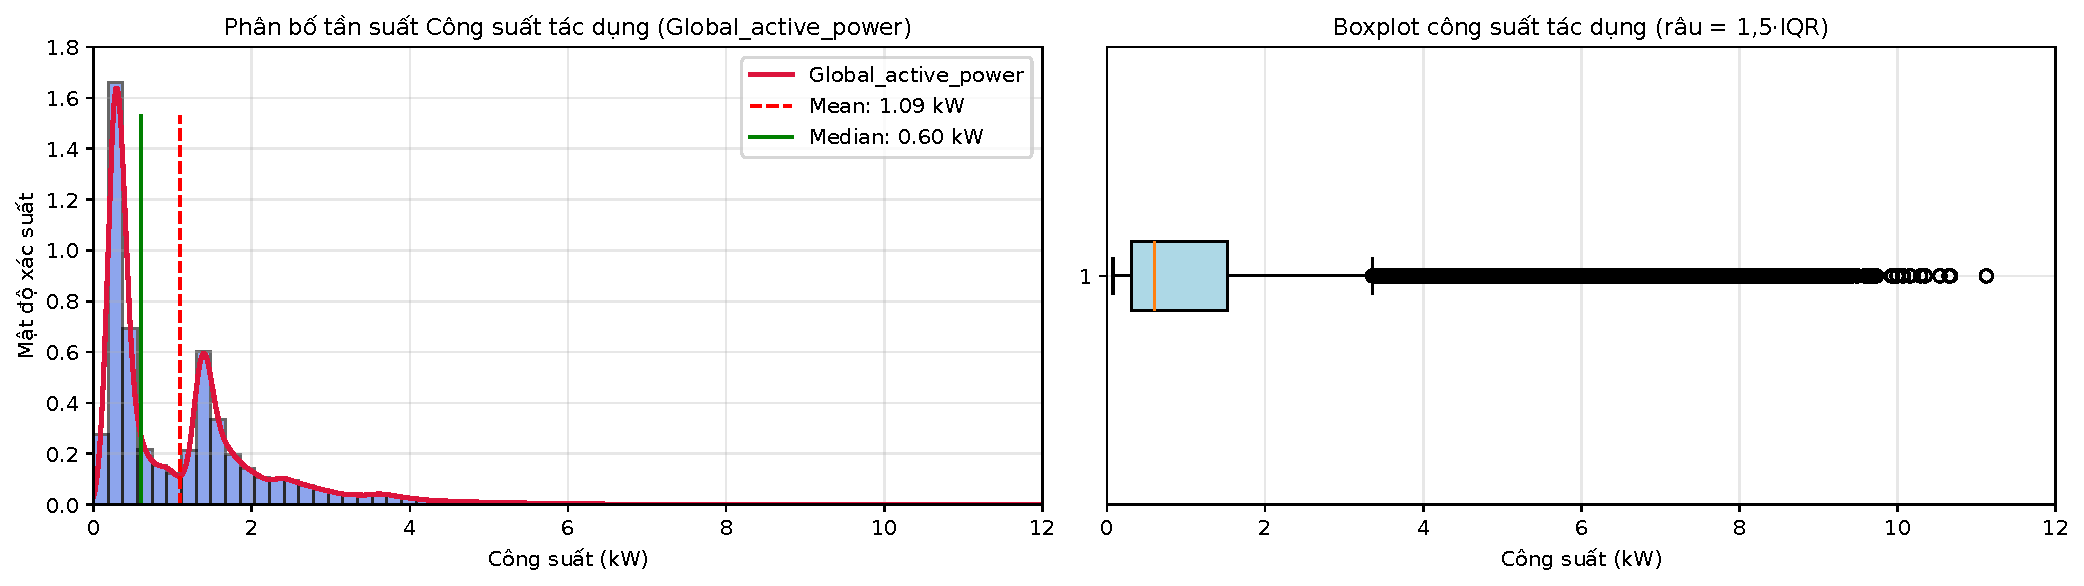
\includegraphics[width=\textwidth]{figures/nb01_gap.pdf}
    \caption{Phân bố công suất tác dụng theo phút: histogram kèm KDE (trái) và biểu đồ hộp với râu 1,5$\cdot$IQR (phải).}
    \label{fig:gap}
\end{figure}

Hình~\ref{fig:gap} cho thấy phân bố công suất lệch phải: khoảng 17,1\% số phút nằm trong vùng tải nền 0,2--0,3 kW. Có 94.907 phút (4,63\%) vượt râu trên 3,358 kW của biểu đồ hộp; đây là các khoảng thời gian tiêu thụ cao kéo dài tới 11,122 kW. Đường KDE tràn nhẹ sang vùng âm là hiệu ứng làm trơn ở biên, không phải dữ liệu âm.

\begin{figure}[htbp]
    \centering
    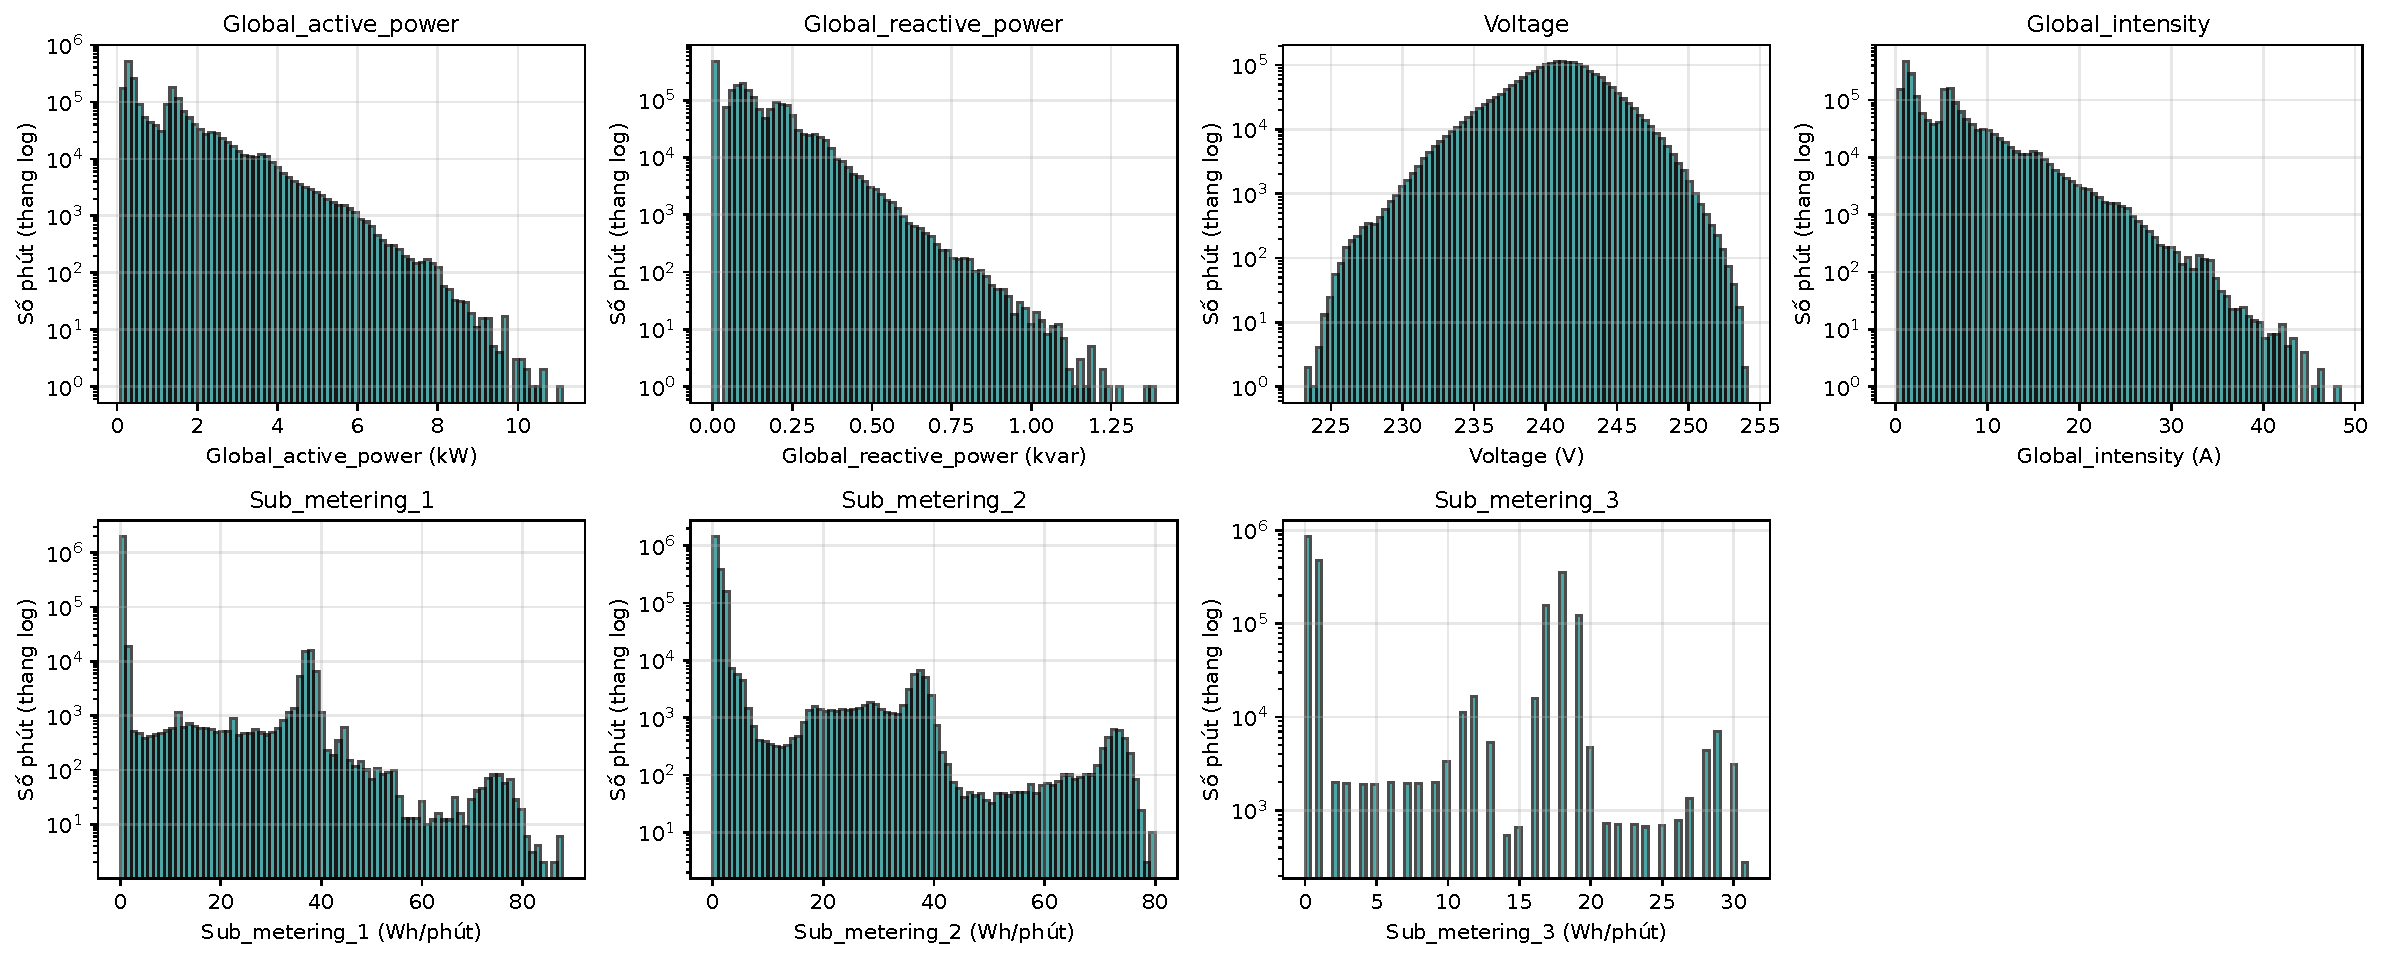
\includegraphics[width=\textwidth]{figures/nb01_bay_bien.pdf}
    \caption{Histogram của bảy biến đo theo phút, trục tung thang logarit.}
    \label{fig:seven}
\end{figure}

Trong Hình~\ref{fig:seven}, công suất tác dụng và cường độ dòng điện có hình dạng gần như giống hệt nhau, là dấu hiệu sớm của tương quan rất cao giữa hai biến. Điện áp có dạng chuông quanh 241 V. \code{Sub_metering_1} và \code{Sub_metering_2} dồn gần hết tại 0, còn \code{Sub_metering_3} có hai cụm tách biệt (0--1 và 17--19 Wh/phút), phù hợp với thiết bị bật/tắt theo bộ ổn nhiệt; đây là giả thuyết vì dữ liệu không cho biết thiết bị nào đang chạy.

\subsection{Nhãn và phân bố nhãn}
\label{sec:label}
Nhãn (điện năng) của một giờ bằng trung bình công suất các phút có đo trong giờ nhân với 1 giờ:
\begin{equation}
    E_{\text{giờ}}\ [\text{kWh}] = \frac{1}{n}\sum_{i=1}^{n} P_i\ [\text{kW}] \times 1\ \text{h},
    \label{eq:energy}
\end{equation}
chỉ tính khi giờ đó có ít nhất 54/60 phút đo; giờ thiếu nhiều hơn được để trống (NaN) và không dùng làm nhãn. Chuỗi theo giờ có 34.589 giờ, trong đó 34.143 giờ hợp lệ (98,71\%). Trên tập huấn luyện (trước 01/01/2010), nhãn có trung bình 1,100 kWh, trung vị 0,794 kWh, độ lệch chuẩn 0,928 kWh và skew 1,31. Phần phân tích phân bố và quan hệ dưới đây chỉ dùng tập huấn luyện để không sử dụng thông tin của tập kiểm tra khi ra quyết định.

\begin{figure}[htbp]
    \centering
    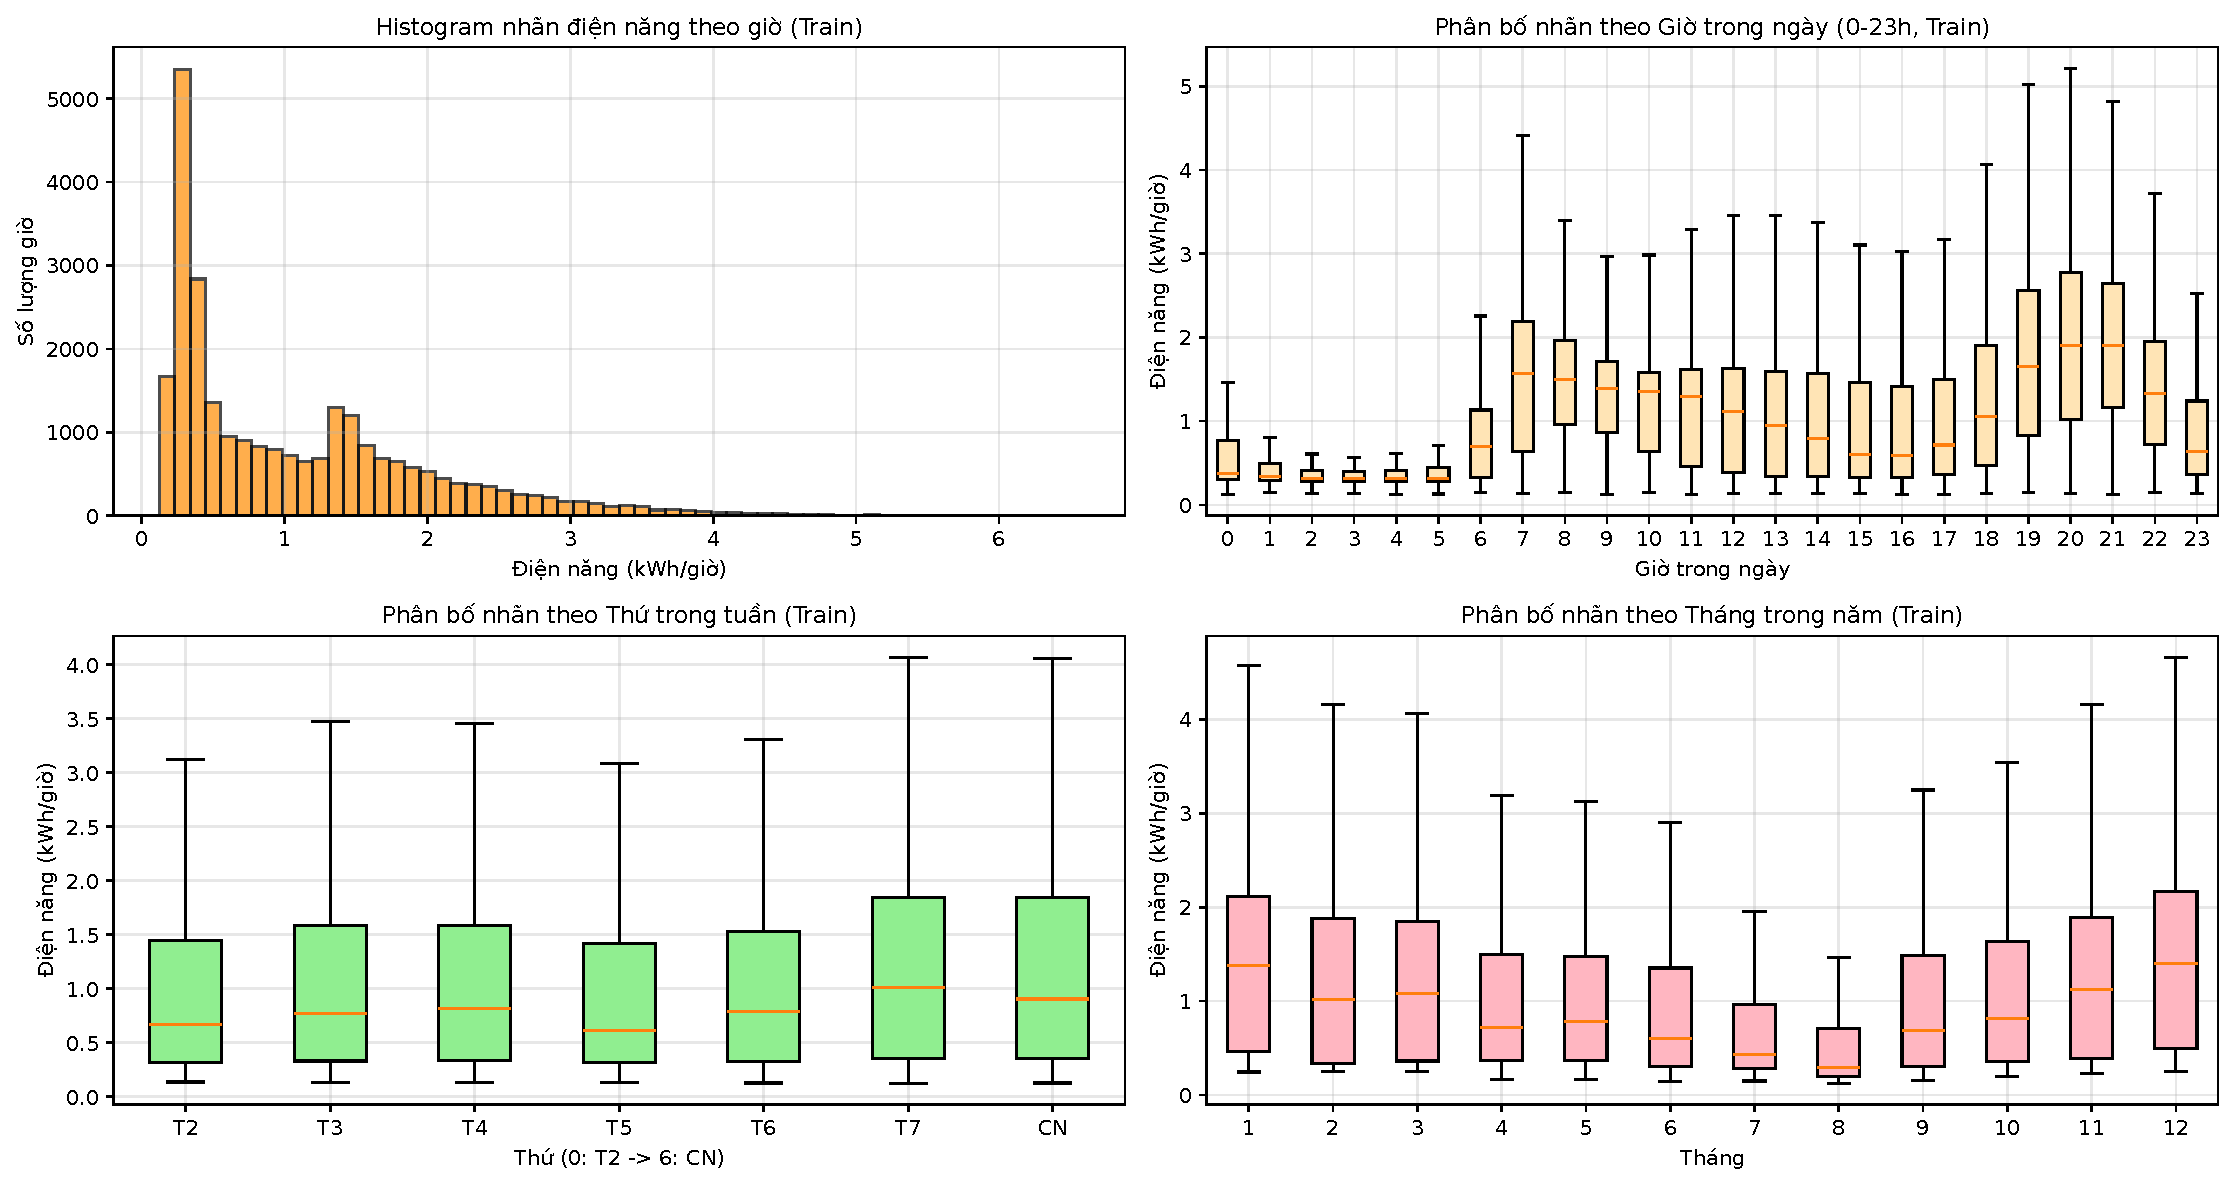
\includegraphics[width=\textwidth]{figures/nb01_nhan.pdf}
    \caption{Phân bố nhãn trên tập huấn luyện: histogram và biểu đồ hộp theo giờ trong ngày, thứ trong tuần, tháng.}
    \label{fig:label}
\end{figure}

Hình~\ref{fig:label} cho thấy bốn đặc điểm của nhãn:
\begin{itemize}
    \item Hai đỉnh: đỉnh chính ở vùng tải nền khoảng 0,23 kWh và đỉnh thứ hai quanh 1,4 kWh.
    \item Chu kỳ ngày: trung vị thấp nhất lúc 3--4 giờ sáng (0,315 kWh), cao nhất lúc 20 giờ (1,904 kWh); khung 19--21 giờ có độ lệch chuẩn lớn nhất (1,10--1,18 kWh), là khung giờ khó dự báo nhất.
    \item Chu kỳ tuần và mùa: trung vị thứ Bảy (1,014) và Chủ nhật (0,904) cao hơn ngày thường (ví dụ thứ Hai 0,665 kWh); tháng 12 cao nhất (1,398 kWh), tháng 8 thấp bất thường (0,289 kWh).
    \item Đuôi phải: chỉ 2,26\% số giờ vượt râu trên 3,494 kWh. Đây là bài toán hồi quy nên không áp dụng cân bằng lớp, nhưng cần theo dõi sai số riêng ở các giờ đỉnh.
\end{itemize}

\subsection{Quan hệ giữa các biến và với nhãn}
\label{sec:correlation}

\begin{figure}[htbp]
    \centering
    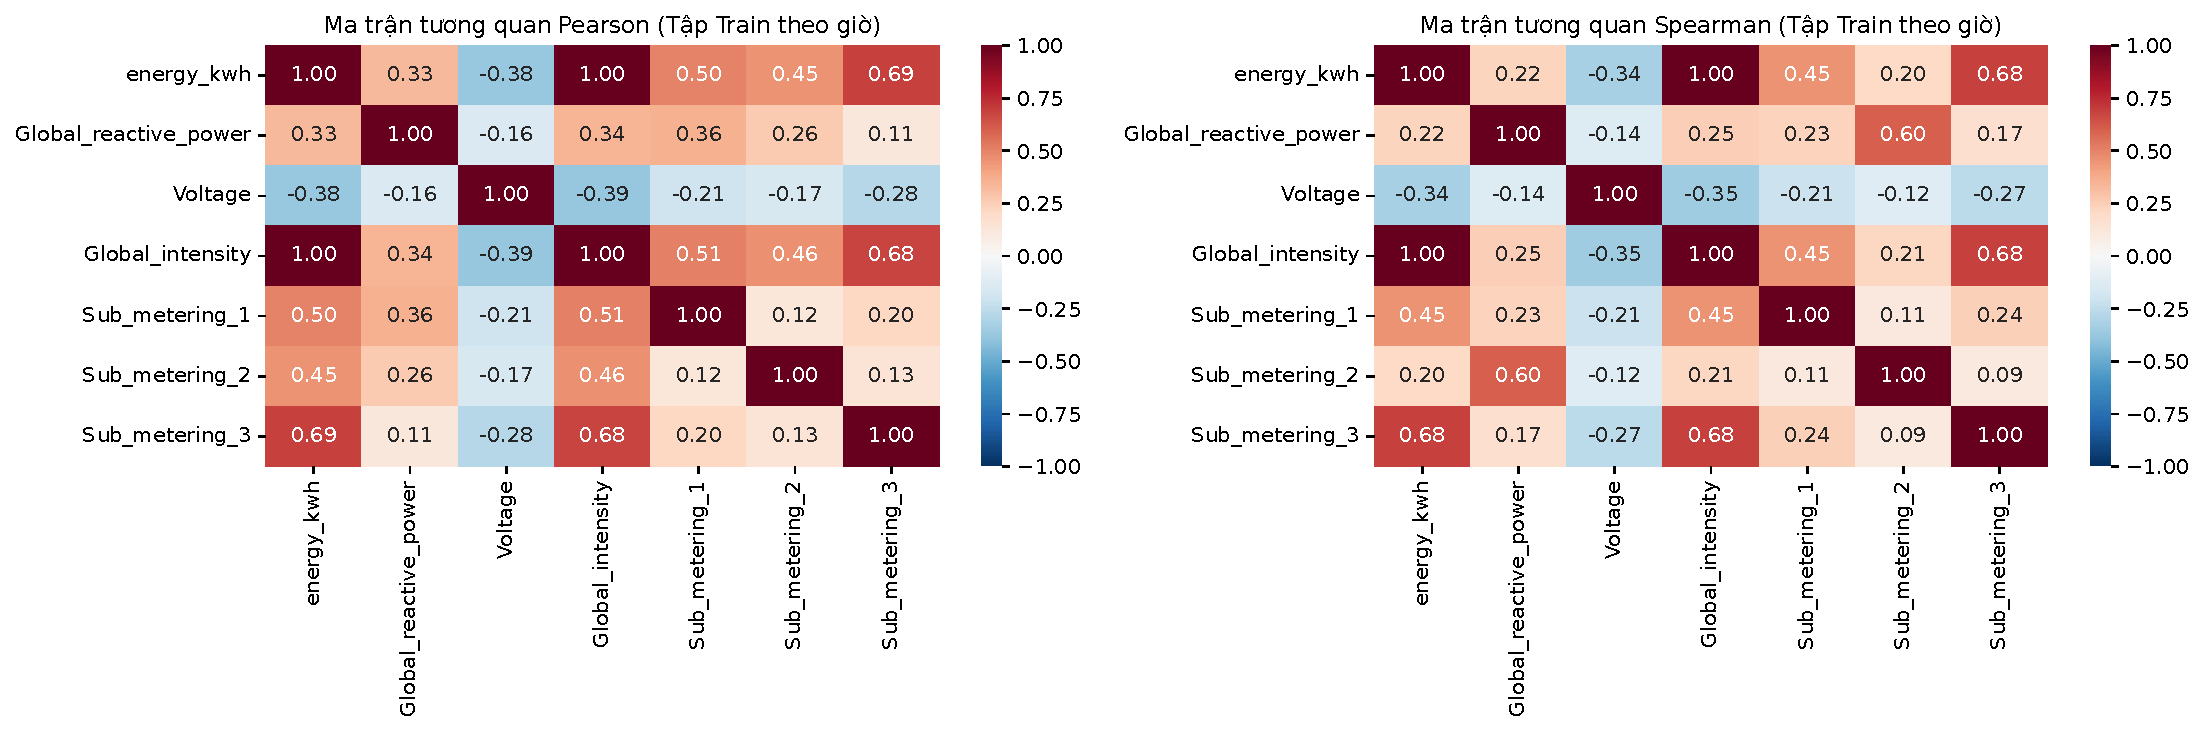
\includegraphics[width=\textwidth]{figures/nb01_tuong_quan.pdf}
    \caption{Ma trận tương quan Pearson (trái) và Spearman (phải) của các biến đo lấy trung bình theo giờ, tập huấn luyện.}
    \label{fig:corr}
\end{figure}

\begin{figure}[htbp]
    \centering
    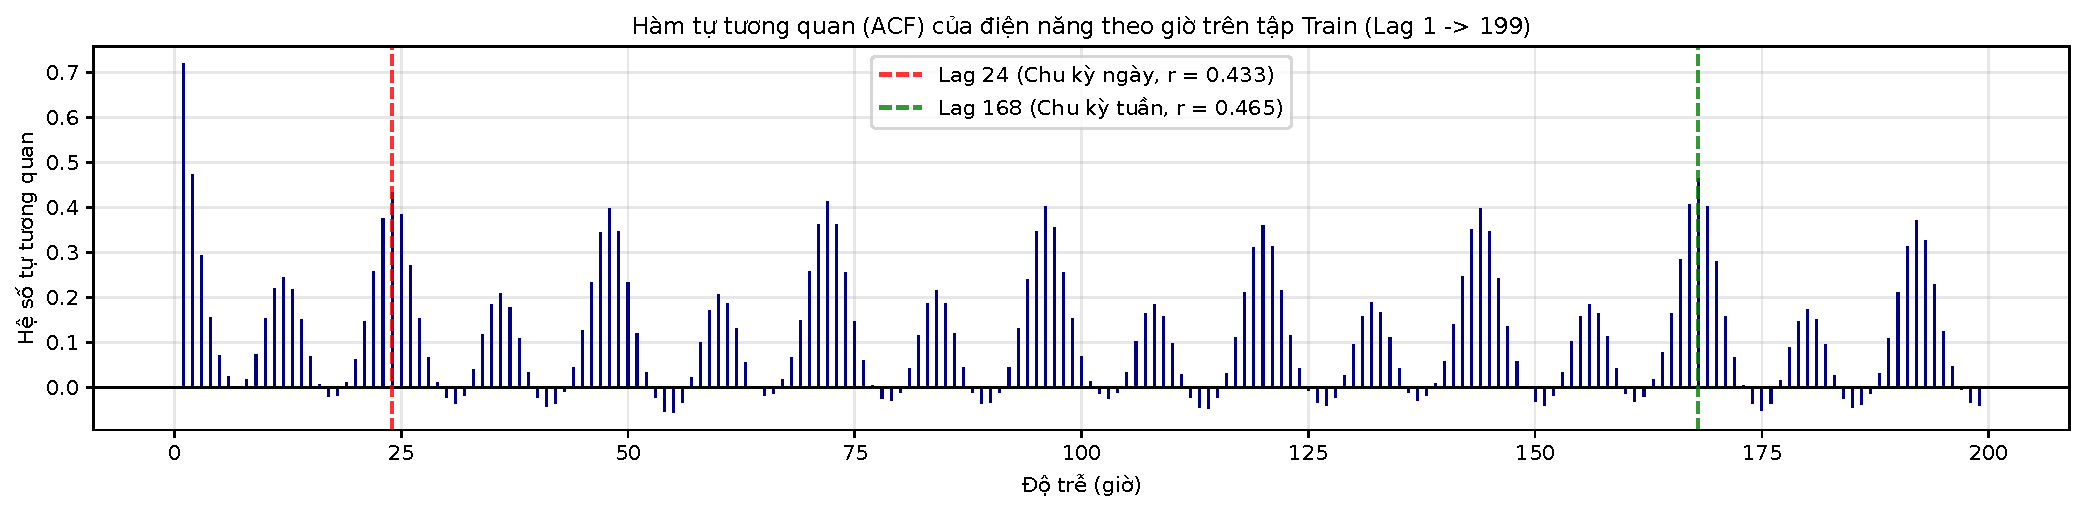
\includegraphics[width=\textwidth]{figures/nb01_acf.pdf}
    \caption{Hàm tự tương quan của điện năng theo giờ trên tập huấn luyện, độ trễ 1--199 giờ.}
    \label{fig:acf}
\end{figure}

Từ Hình~\ref{fig:corr} và Hình~\ref{fig:acf}, nhóm rút ra bốn nhận xét có ý nghĩa cho việc xây dựng mô hình:
\begin{enumerate}
    \item Rò rỉ qua cường độ dòng điện. Tương quan giữa \code{Global_intensity} và nhãn là 0,999 (Pearson) và 0,998 (Spearman), vì công suất xấp xỉ bằng điện áp nhân cường độ. Đại lượng này đo cùng lúc với nhãn nên không có tại thời điểm dự báo; nhóm loại nó, cùng với \code{Voltage} của thời điểm mục tiêu.
    \item Tương quan giảm nhanh rồi tăng lại theo chu kỳ. Tự tương quan giảm từ 0,719 ở độ trễ 1 xuống 0,023 ở độ trễ 6, rồi tăng lại ở 24 giờ (0,433) và 168 giờ (0,465). Vì vậy với $h \ge 6$, thông tin chủ yếu đến từ giá trị cùng giờ ngày trước và tuần trước của thời điểm mục tiêu, không phải từ các giờ gần nhất.
    \item Quan hệ giữa giờ trong ngày và nhãn không đơn điệu (thấp ban đêm, tăng buổi sáng, đỉnh buổi tối). Mô hình tuyến tính cần mã hóa one-hot cho giờ; mô hình cây có thể tự học quan hệ này.
    \item Nhóm công tơ phụ và điện áp. \code{Sub_metering_3} tương quan cao nhất với nhãn trong ba nhóm (0,687) nhưng là giá trị cùng thời điểm, nên chỉ có thể dùng giá trị trễ của nó. Điện áp tương quan âm với nhãn ($-0{,}375$): giờ tiêu thụ cao thường có điện áp thấp hơn.
\end{enumerate}

\subsection{Tính mùa vụ theo ngày}

\begin{figure}[htbp]
    \centering
    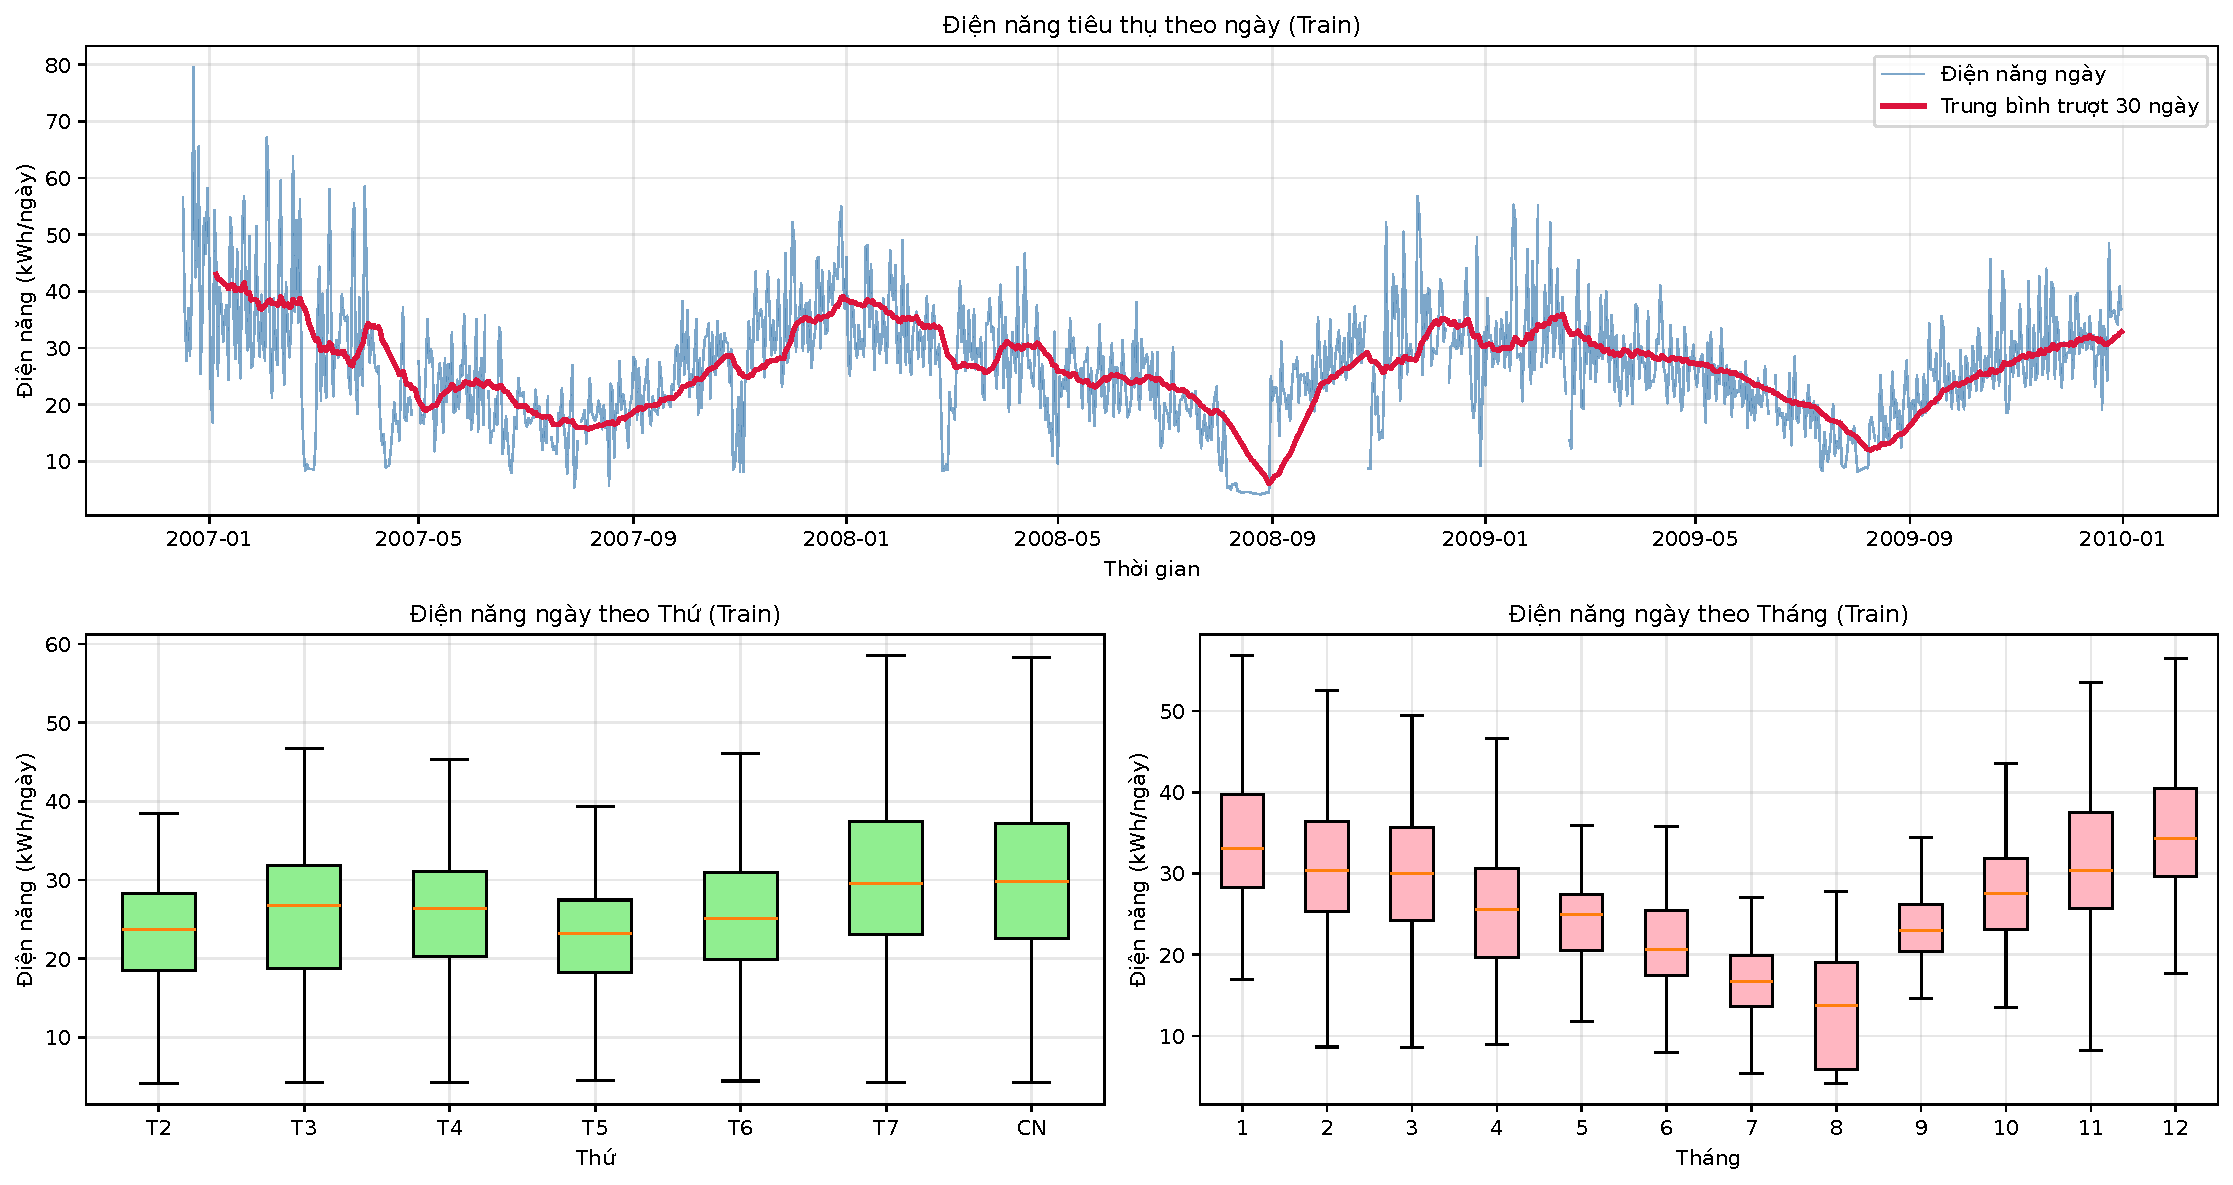
\includegraphics[width=\textwidth]{figures/nb01_theo_ngay.pdf}
    \caption{Điện năng theo ngày trên tập huấn luyện: chuỗi ngày kèm trung bình trượt 30 ngày (trên), biểu đồ hộp theo thứ và theo tháng (dưới).}
    \label{fig:daily}
\end{figure}

Điện năng ngày là tổng 24 giờ; chỉ giữ các ngày đủ 24 giờ hợp lệ (31 trên 1.442 ngày bị loại). Hình~\ref{fig:daily} cho thấy mùa vụ theo năm rõ rệt: trung vị tháng 12 (34,31 kWh/ngày) gấp khoảng 2,5 lần tháng 8 (13,79 kWh/ngày); tự tương quan của chuỗi ngày ở độ trễ 364 ngày là 0,537. Chu kỳ tuần cũng xuất hiện: tự tương quan ở độ trễ 7 ngày (0,554) cao hơn ở 6 ngày (0,499), cuối tuần tiêu thụ cao hơn ngày thường. Nguyên nhân tháng 8 thấp (có thể là kỳ nghỉ hè) không kiểm chứng được từ dữ liệu.

\section{Chất lượng dữ liệu và xử lý}
\label{sec:quality}

\subsection{Định lượng các vấn đề chất lượng}
Bảng~\ref{tab:quality} tổng hợp kết quả kiểm tra chất lượng dữ liệu.

\begin{table}[htbp]
    \centering
    \caption{Các vấn đề chất lượng dữ liệu đã định lượng.}
    \label{tab:quality}
    \small
    \begin{tabularx}{\textwidth}{|>{\raggedright\arraybackslash}p{3.2cm}|>{\raggedright\arraybackslash}X|>{\raggedright\arraybackslash}p{4.0cm}|}
        \hline
        \textbf{Vấn đề} & \textbf{Định lượng} & \textbf{Ảnh hưởng} \\ \hline
        Sai định dạng & 155.874 ký tự ``?'' ở 6 cột số & Cột bị đọc thành chuỗi \\ \hline
        Bản ghi trùng & 0 mốc thời gian trùng; 0 mốc bị thiếu trên lưới 1 phút & Không có \\ \hline
        Giá trị thiếu & 25.979 dòng (1,252\%), cả 25.979 dòng thiếu đồng thời 7 biến & Mất thông tin ở các khoảng thiếu \\ \hline
        Thiếu dạng khối & 71 khối liên tục; 6 khối dài hơn 1 ngày chiếm 94,9\% số phút thiếu; khối dài nhất 120,4 giờ từ 17/08/2010; 4 trong 6 khối dài thuộc năm 2010 & Không phù hợp nội suy; tập kiểm tra bị ảnh hưởng nhiều hơn \\ \hline
        Ngoại lai (1,5$\cdot$IQR) & Công suất: 94.907 phút (4,63\%); \code{Sub_metering_1}: 8,25\% & Là các giờ tiêu thụ cao có thật \\ \hline
        Tính hợp lý vật lý & 0 giá trị âm; 57 phút điện áp trên 253 V (0,003\%) & Không thấy giá trị phi vật lý \\ \hline
        Nhất quán đơn vị & 0,05\% số phút có điện năng ``còn lại'' âm (nhỏ nhất $-2{,}4$ Wh/phút) & Rất nhỏ, có thể do làm tròn \\ \hline
        Nguy cơ rò rỉ & Tương quan giữa công suất và $V \cdot I$ là 0,99909 & Loại \code{Global_intensity} \\ \hline
        Mất cân bằng & 2,26\% số giờ huấn luyện vượt râu trên 3,494 kWh & Theo dõi sai số ở giờ đỉnh \\ \hline
    \end{tabularx}
\end{table}

\begin{figure}[htbp]
    \centering
    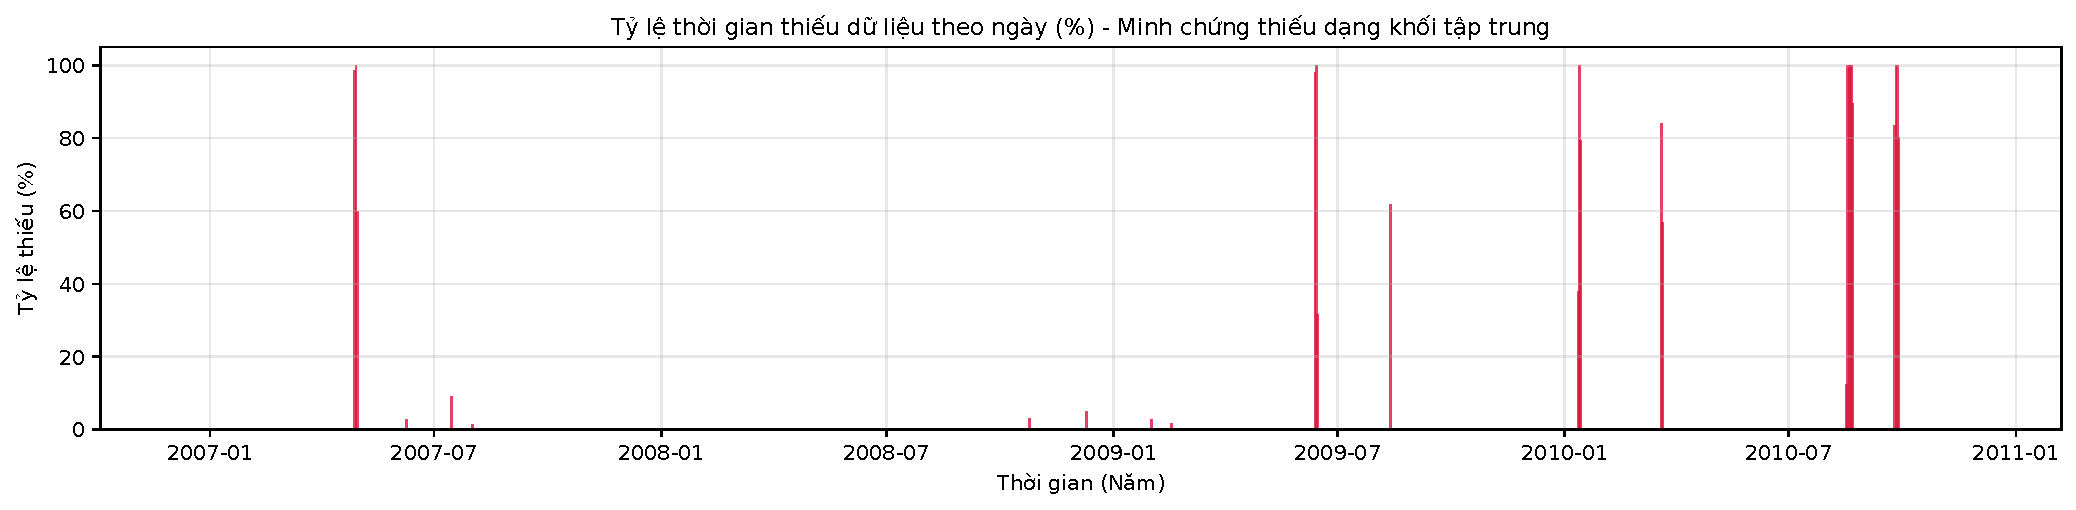
\includegraphics[width=\textwidth]{figures/nb01_thieu_theo_ngay.pdf}
    \caption{Tỷ lệ phút thiếu dữ liệu theo ngày.}
    \label{fig:missing}
\end{figure}

Hình~\ref{fig:missing} cho thấy dữ liệu thiếu không rải rác từng phút mà tập trung thành các khối kéo dài nhiều ngày. Mô hình thiếu này không phù hợp với giả định thiếu hoàn toàn ngẫu nhiên (MCAR)~\cite{little2019statistical}; nguyên nhân có thể là thiết bị ghi bị ngắt, nhưng dữ liệu không cho biết.

\subsection{Phương án xử lý}
Bảng~\ref{tab:treatment} nêu cách xử lý từng vấn đề và lý do lựa chọn.

\begin{table}[htbp]
    \centering
    \caption{Phương án xử lý các vấn đề chất lượng dữ liệu.}
    \label{tab:treatment}
    \small
    \begin{tabularx}{\textwidth}{|>{\raggedright\arraybackslash}p{2.6cm}|>{\raggedright\arraybackslash}p{4.3cm}|>{\raggedright\arraybackslash}X|}
        \hline
        \textbf{Vấn đề} & \textbf{Cách xử lý} & \textbf{Lý do} \\ \hline
        Ký tự ``?'' & Đọc là giá trị thiếu, ép kiểu số thực & ``?'' là ký hiệu thiếu của nguồn; không thay bằng 0 vì hộ luôn có tải nền. \\ \hline
        Thiếu ở nhãn & Tổng hợp theo giờ; giờ có dưới 54 phút đo để NaN; không nội suy, không xóa dòng & Nội suy qua khối thiếu dài tới 5 ngày sẽ tạo nhãn giả từ dữ liệu sau khối. Giữ NaN trên lưới giờ để phép dịch $k$ dòng luôn đúng $k$ giờ. \\ \hline
        Thiếu ở đặc trưng & Điền trung vị trong Pipeline, chỉ học trên tập huấn luyện & Trung vị ít bị kéo bởi giờ đỉnh hơn trung bình khi phân bố lệch phải. \\ \hline
        Ngoại lai & Giữ nguyên & Không có giá trị âm hay vượt ngưỡng vật lý; giờ tiêu thụ cao là đối tượng cần dự báo. \\ \hline
        Rò rỉ & Loại \code{Global_intensity}, \code{Voltage} của thời điểm mục tiêu & Không biết được tại thời điểm dự báo. \\ \hline
        Mất cân bằng & Không sinh mẫu nhân tạo & Sinh mẫu phá vỡ cấu trúc thời gian; thay bằng phân tích sai số theo giờ và theo dải giá trị. \\ \hline
    \end{tabularx}
\end{table}

Ngưỡng 54/60 phút được chọn sau khi thử các ngưỡng khác: đổi ngưỡng từ 60 xuống 1 phút chỉ làm số giờ hợp lệ thay đổi 83 giờ (từ 34.085 lên 34.168), vì phần lớn giờ thiếu là thiếu trọn vẹn (421 giờ không có phút nào). Ngưỡng 54 phút giữ thêm 58 giờ so với ngưỡng 60 mà vẫn bảo đảm trung bình được tính trên ít nhất 90\% thời gian của giờ.

\subsection{So sánh trước và sau xử lý}

\begin{table}[htbp]
    \centering
    \caption{So sánh công suất theo phút (trước) và điện năng theo giờ (sau xử lý).}
    \label{tab:before_after}
    \small
    \begin{tabular}{|l|r|r|}
        \hline
        \textbf{Chỉ số} & \textbf{Trước: công suất theo phút (kW)} & \textbf{Sau: điện năng theo giờ (kWh)} \\ \hline
        Số dòng & 2.075.259 & 34.589 \\ \hline
        Số dòng thiếu (tỷ lệ) & 25.979 (1,252\%) & 446 (1,289\%) \\ \hline
        Trung bình & 1,092 & 1,092 \\ \hline
        Độ lệch chuẩn & 1,057 & 0,898 \\ \hline
        Trung vị & 0,602 & 0,803 \\ \hline
        Min / Max & 0,076 / 11,122 & 0,124 / 6,561 \\ \hline
        Skew & 1,79 & 1,30 \\ \hline
    \end{tabular}
\end{table}

\begin{figure}[htbp]
    \centering
    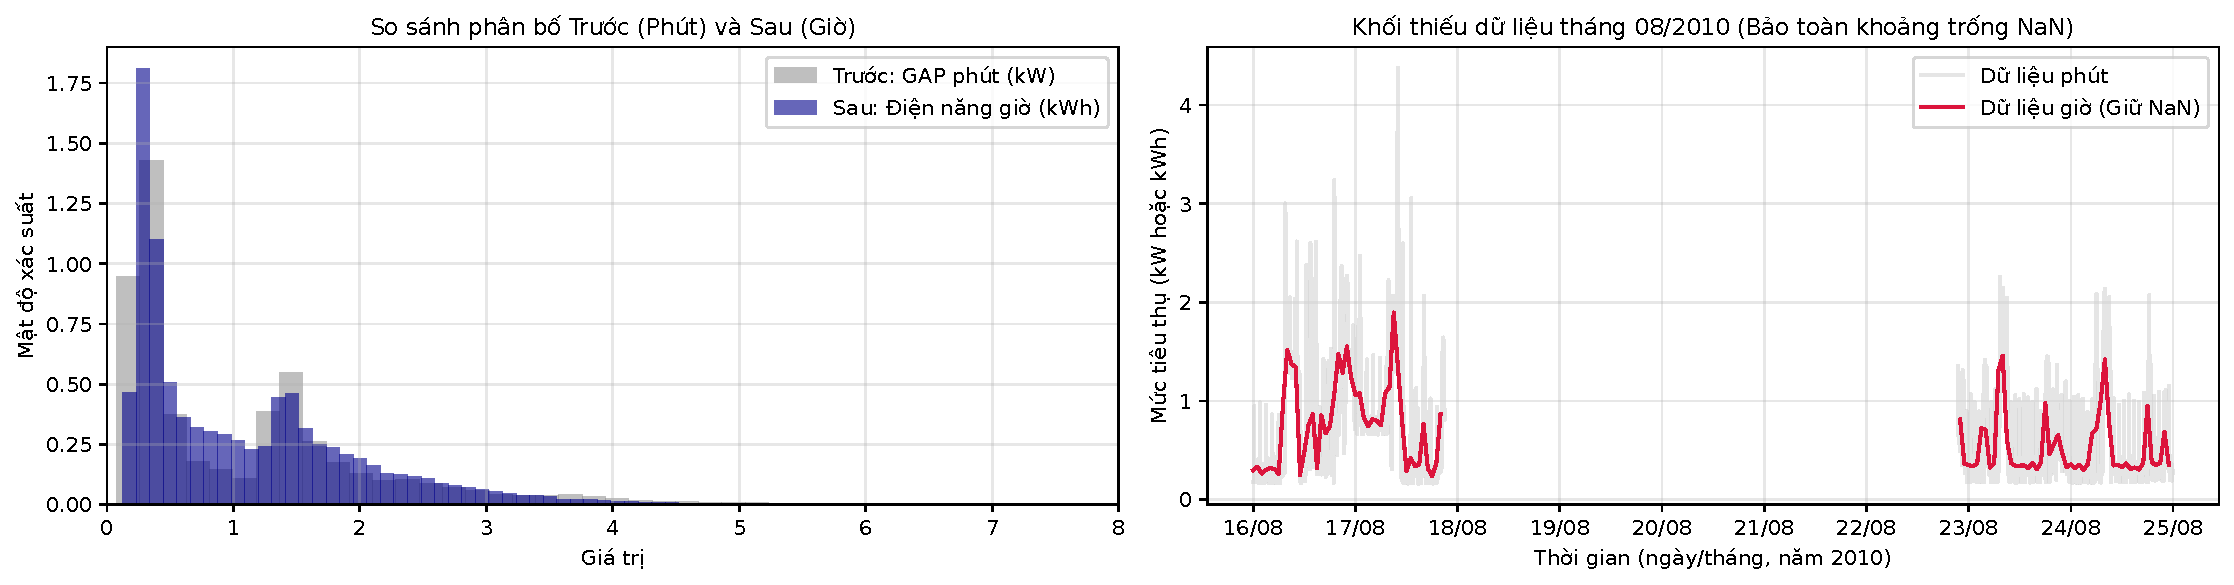
\includegraphics[width=\textwidth]{figures/nb01_truoc_sau.pdf}
    \caption{Phân bố trước và sau xử lý (trái); đoạn chứa khối thiếu dài nhất tháng 8/2010, khối thiếu được giữ nguyên (phải).}
    \label{fig:before_after}
\end{figure}

Bảng~\ref{tab:before_after} và Hình~\ref{fig:before_after} cho thấy trung bình giữ nguyên 1,092 (điện năng được bảo toàn khi gộp theo giờ), còn độ lệch chuẩn giảm 15\%, giá trị lớn nhất giảm từ 11,122 xuống 6,561 và skew giảm từ 1,79 xuống 1,30, do các đỉnh kéo dài vài phút được trung bình hóa trong giờ. Khối thiếu tháng 8/2010 được để trống thay vì nối bằng một đoạn thẳng giả.

\section{Chuẩn bị dữ liệu cho mô hình}
\label{sec:preparation}

\subsection{Chia dữ liệu theo thời gian}
Dữ liệu được chia theo thời điểm mục tiêu $t+h$, không xáo trộn: mẫu có nhãn trước 01/01/2010 thuộc tập huấn luyện, từ 01/01/2010 thuộc tập kiểm tra. Chia theo thời điểm mục tiêu (thay vì thời điểm gốc) bảo đảm không có nhãn nào của năm 2010 lọt vào tập huấn luyện, kể cả khi $h = 24$. Với $h = 1$, tập huấn luyện có 26.523 mẫu (nhãn từ 16/12/2006 đến 31/12/2009, 77,7\%) và tập kiểm tra có 7.620 mẫu (từ 01/01/2010 đến 26/11/2010, 22,3\%). Tập kiểm tra được giữ riêng: không dùng để khảo sát, chọn đặc trưng hay chọn mô hình.

\subsection{Kiểm định chéo theo thời gian}
Trên tập huấn luyện, nhóm dùng TimeSeriesSplit với 5 fold, mỗi fold kiểm định dài 2.160 giờ (90 ngày) và khoảng đệm 168 mẫu (một tuần) giữa phần huấn luyện và phần kiểm định~\cite{sklearn2026tss}.

\begin{table}[htbp]
    \centering
    \caption{Các fold kiểm định chéo với $h = 1$ (mọi fold huấn luyện bắt đầu từ 16/12/2006).}
    \label{tab:folds}
    \small
    \begin{tabular}{|c|r|c|r|c|}
        \hline
        \textbf{Fold} & \textbf{Mẫu huấn luyện} & \textbf{Huấn luyện đến} & \textbf{Mẫu kiểm định} & \textbf{Khoảng kiểm định} \\ \hline
        1 & 15.555 & 27/09/2008 & 2.160 & 04/10/2008 -- 02/01/2009 \\ \hline
        2 & 17.715 & 26/12/2008 & 2.160 & 02/01/2009 -- 03/04/2009 \\ \hline
        3 & 19.875 & 27/03/2009 & 2.160 & 03/04/2009 -- 04/07/2009 \\ \hline
        4 & 22.035 & 27/06/2009 & 2.160 & 04/07/2009 -- 02/10/2009 \\ \hline
        5 & 24.195 & 25/09/2009 & 2.160 & 03/10/2009 -- 31/12/2009 \\ \hline
    \end{tabular}
\end{table}

\begin{figure}[htbp]
    \centering
    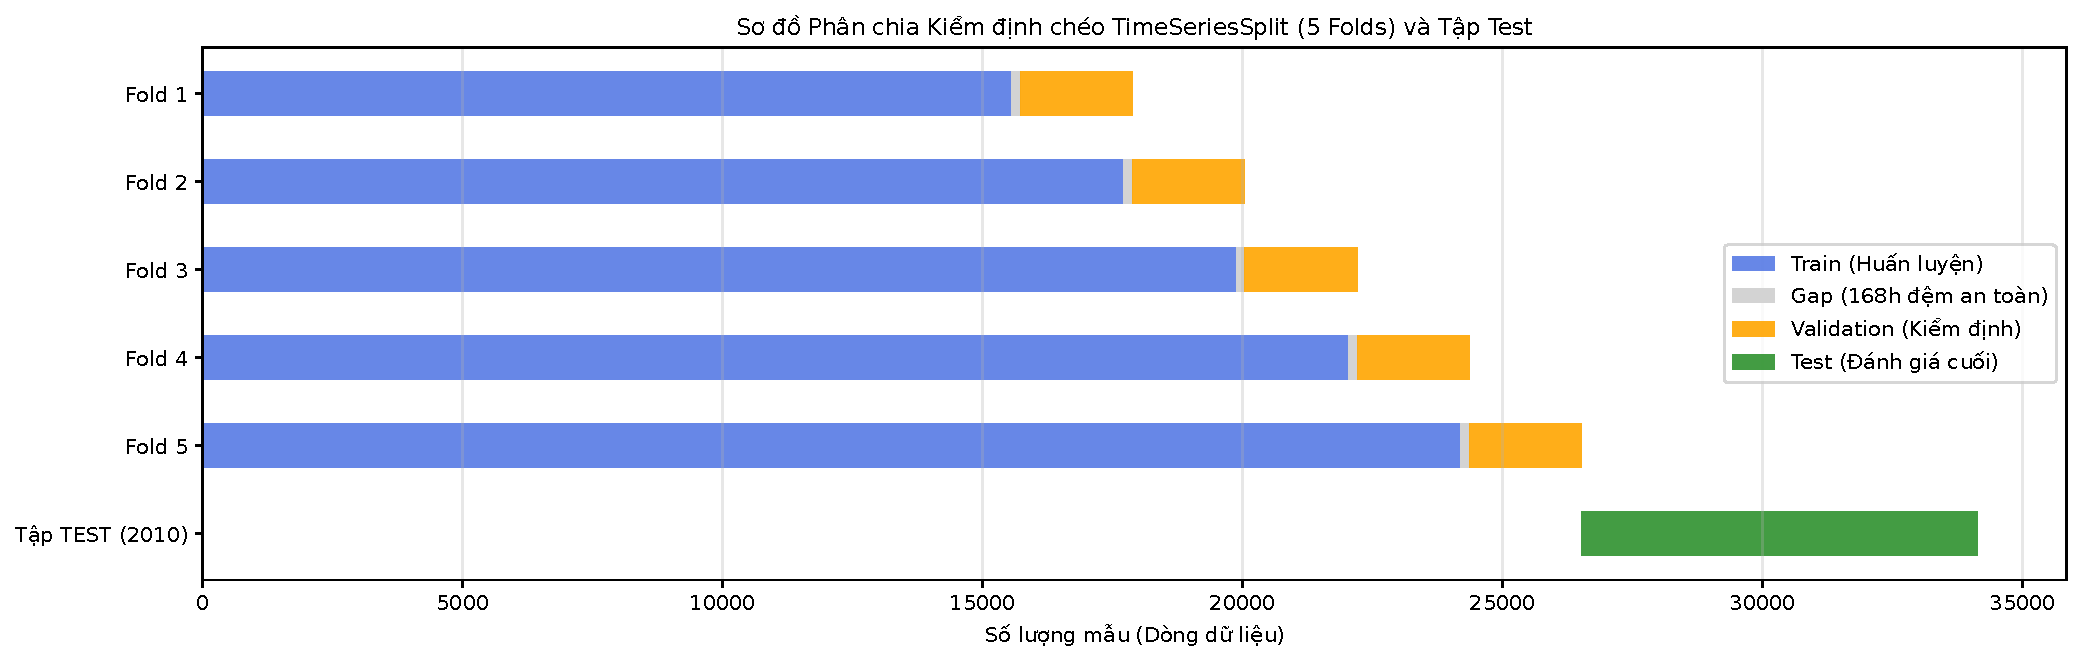
\includegraphics[width=\textwidth]{figures/nb02_fold.pdf}
    \caption{Sơ đồ 5 fold TimeSeriesSplit và tập kiểm tra; trục hoành là chỉ số mẫu.}
    \label{fig:folds}
\end{figure}

Như Bảng~\ref{tab:folds} và Hình~\ref{fig:folds}, các fold kiểm định có cùng kích thước, nối tiếp và không chồng nhau; phần huấn luyện mở rộng thêm 2.160 mẫu mỗi fold. Khoảng đệm bảo đảm nhãn của các mẫu huấn luyện cuối cùng không trùng khoảng thời gian với nhãn của các mẫu kiểm định đầu tiên khi $h \le 24$, đồng thời giảm phụ thuộc do tự tương quan giữa hai phần. Các fold kiểm định rơi vào các mùa khác nhau, nên chênh lệch sai số giữa các fold phản ánh cả mùa vụ; kết quả vì vậy được báo cáo bằng trung bình $\pm$ độ lệch chuẩn qua 5 fold.

\subsection{Đường ống tiền xử lý}
Các bước tiền xử lý được tổ chức thành một Pipeline của thư viện scikit-learn~\cite{pedregosa2011scikit}: biến giờ trong ngày được mã hóa one-hot, các đặc trưng số được điền khuyết bằng trung vị rồi chuẩn hóa z-score. Đường ống chỉ được khớp (fit) trên dữ liệu huấn luyện; với $h = 1$, giá trị học được cho đặc trưng $y_t$ là trung vị 0,7939, trung bình 1,1002 và độ lệch chuẩn 0,9278 kWh.

\begin{figure}[htbp]
    \centering
    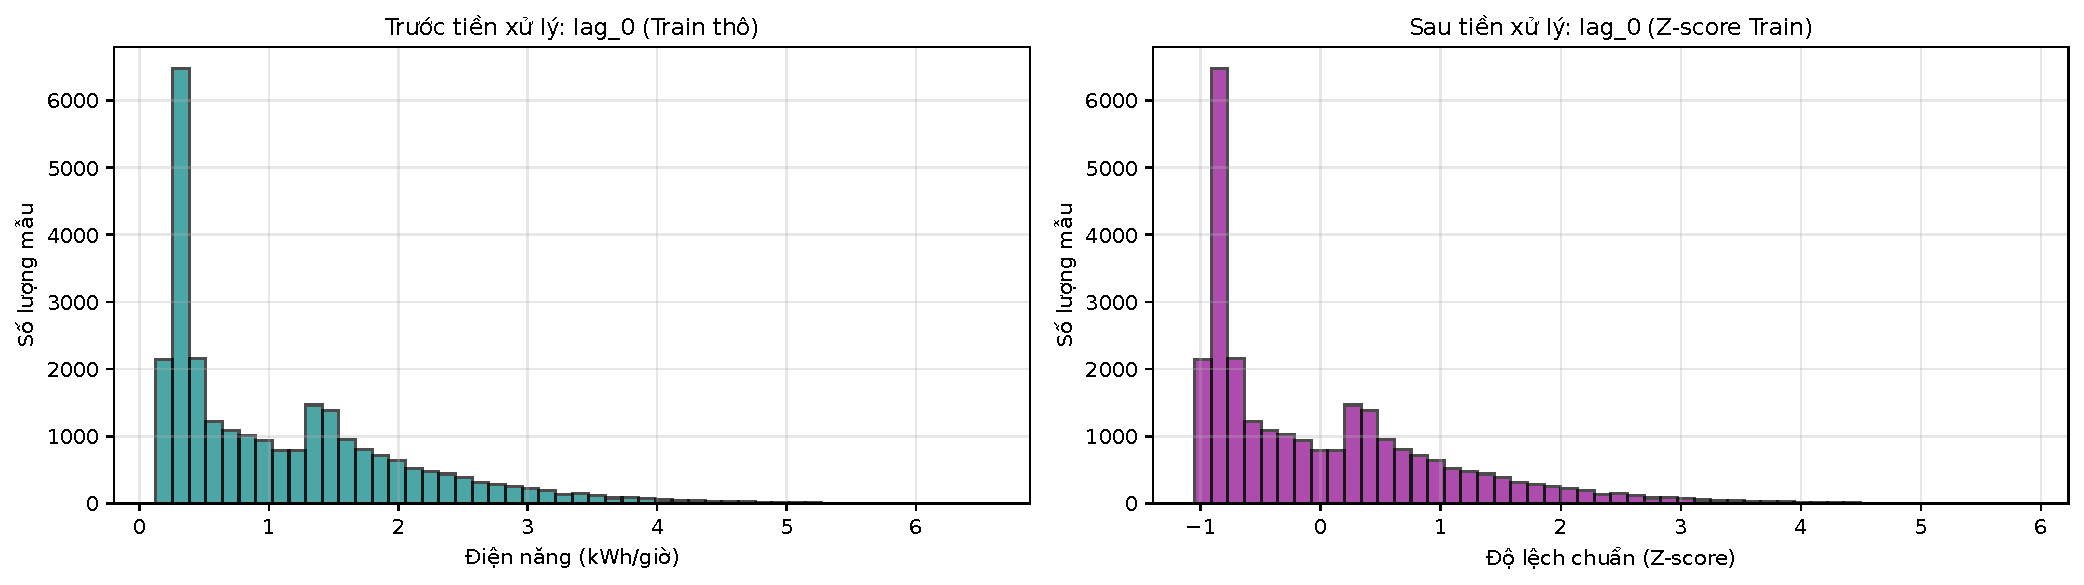
\includegraphics[width=\textwidth]{figures/nb02_chuan_hoa.pdf}
    \caption{Phân bố của đặc trưng $y_t$ trên tập huấn luyện trước và sau tiền xử lý.}
    \label{fig:scaling}
\end{figure}

Sau tiền xử lý, số giá trị thiếu ở cả hai tập về 0. Trên tập huấn luyện, các đặc trưng số có trung bình 0 và độ lệch chuẩn 1; trên tập kiểm tra, trung bình khoảng $-0{,}04$ và độ lệch chuẩn khoảng 0,84, vì năm 2010 tiêu thụ thấp và ít biến động hơn giai đoạn huấn luyện. Điều này cho thấy tập kiểm tra không bị dùng để học tham số chuẩn hóa. Hình~\ref{fig:scaling} cho thấy chuẩn hóa chỉ dịch và co giãn trục, không đổi hình dạng phân bố. Để minh họa rò rỉ, nhóm so sánh với cách khớp trên toàn bộ dữ liệu: trung bình học được của $y_t$ giảm từ 1,1004 xuống 1,0916 và độ lệch chuẩn giảm khoảng 0,03, tức thông tin của năm 2010 đã lọt vào tham số chuẩn hóa.

\chapter{XÂY DỰNG VÀ ĐÁNH GIÁ MÔ HÌNH}
\label{chap:models}

Chương này trình bày bộ đặc trưng, lý do lựa chọn thuật toán, quy trình huấn luyện và kiểm định chéo, kết quả so sánh các mô hình với mô hình cơ sở, phân tích lỗi và các đặc trưng ảnh hưởng nhiều đến dự báo. Ở giai đoạn này, tập kiểm tra năm 2010 chưa được sử dụng; mọi kết quả là kết quả kiểm định chéo trên tập huấn luyện.

\section{Bộ đặc trưng}
\label{sec:features}

Với mỗi tầm dự báo $h$, bảng có giám sát gồm 21 đặc trưng chỉ dùng thông tin đến thời điểm gốc $t$ (Bảng~\ref{tab:features}). Các đặc trưng được chọn dựa trên kết quả khảo sát ở Chương~\ref{chap:data}.

\begin{table}[htbp]
    \centering
    \caption{Bộ đặc trưng dùng cho mô hình.}
    \label{tab:features}
    \small
    \begin{tabularx}{\textwidth}{|>{\raggedright\arraybackslash}p{2.6cm}|>{\raggedright\arraybackslash}p{5.6cm}|>{\raggedright\arraybackslash}X|}
        \hline
        \textbf{Nhóm} & \textbf{Đặc trưng} & \textbf{Căn cứ} \\ \hline
        Trễ (9) & $y_{t-k}$, $k \in \{0,1,2,3,5,11,23,47,167\}$ & Tự tương quan cao ở vài giờ gần nhất và ở 24, 168 giờ (Hình~\ref{fig:acf}) \\ \hline
        Cùng giờ của mục tiêu (2) & $y_{t+h-24}$ (cùng giờ ngày trước), $y_{t+h-168}$ (cùng giờ tuần trước) & Chu kỳ ngày và tuần; cũng là đầu vào của SNaive24, SNaive168 \\ \hline
        Cửa sổ trượt (6) & Trung bình và độ lệch chuẩn của 3, 24, 168 giờ gần nhất, kết thúc tại $t$ & Mức nền và độ biến động gần đây \\ \hline
        Lịch (4) & Giờ, thứ, tháng, cờ cuối tuần của thời điểm mục tiêu $t+h$ & Mùa vụ theo giờ, tuần, năm (Hình~\ref{fig:label}, \ref{fig:daily}) \\ \hline
    \end{tabularx}
\end{table}

Notebook kiểm tra trực tiếp rằng bộ đặc trưng không dùng thông tin tương lai: thay toàn bộ giá trị sau một mốc $T$ bằng một giá trị vô lý, các đặc trưng tại mọi thời điểm $t \le T$ không thay đổi.

\section{Lựa chọn thuật toán}
\label{sec:algorithms}

Nhóm dùng bốn mô hình cơ sở theo~\eqref{eq:baselines}: Mean (trung bình nhãn của phần huấn luyện), Naive, SNaive24 và SNaive168. Ba mô hình học máy được chọn theo định hướng của đề tài và đặc điểm dữ liệu (Bảng~\ref{tab:algorithms}).

\begin{table}[htbp]
    \centering
    \caption{Lý do lựa chọn và cấu hình các mô hình học máy.}
    \label{tab:algorithms}
    \small
    \begin{tabularx}{\textwidth}{|>{\raggedright\arraybackslash}p{2.5cm}|>{\raggedright\arraybackslash}X|>{\raggedright\arraybackslash}p{4.6cm}|}
        \hline
        \textbf{Mô hình} & \textbf{Lý do lựa chọn} & \textbf{Tiền xử lý và siêu tham số} \\ \hline
        Linear Regression & Mô hình tham số đơn giản nhất, dễ diễn giải; kiểm tra phần quan hệ tuyến tính giữa nhãn và các giá trị trễ. & One-hot giờ, thứ, tháng (bỏ một mức mỗi nhóm); điền trung vị và chuẩn hóa cột số. \\ \hline
        Random Forest & Học được quan hệ phi tuyến và tương tác giờ $\times$ thứ $\times$ tháng mà khảo sát đã chỉ ra; lấy trung bình nhiều cây giúp giảm phương sai. & Điền trung vị; 300 cây; tối thiểu 5 mẫu ở mỗi lá; mỗi lần tách xét 50\% số đặc trưng. \\ \hline
        XGBoost & Boosting cây thường cho sai số thấp trên dữ liệu dạng bảng khoảng vài chục nghìn mẫu; xử lý trực tiếp giá trị thiếu sau các khối dữ liệu thiếu. & 400 cây; tốc độ học 0,05; độ sâu tối đa 6; tổng trọng số tối thiểu ở lá 5; mỗi cây dùng 80\% số mẫu và 80\% số đặc trưng. \\ \hline
    \end{tabularx}
\end{table}

Siêu tham số được cố định trước ở các giá trị phổ biến và không được chọn theo kết quả kiểm định. Việc dò tìm siêu tham số trên kiểm định chéo thuộc giai đoạn tối ưu hóa ở bước tiếp theo; tách hai giai đoạn giúp đo được tác động của việc tối ưu. Mọi mô hình cố định hạt giống ngẫu nhiên bằng 42 để kết quả tái lập được.

\section{Quy trình huấn luyện và đánh giá}
\label{sec:protocol}

Mỗi mô hình học máy được tổ chức thành một Pipeline gồm các bước tiền xử lý và mô hình. Quy trình kiểm định chéo trên tập huấn luyện như sau:
\begin{enumerate}
    \item Dùng 5 fold TimeSeriesSplit như Bảng~\ref{tab:folds}; mỗi tầm dự báo $h$ huấn luyện một mô hình riêng.
    \item Ở mỗi fold, Pipeline được khớp lại chỉ trên phần huấn luyện của fold đó, nên giá trị điền khuyết và tham số chuẩn hóa không chứa thông tin của phần kiểm định.
    \item Mọi mô hình được chấm trên cùng tập mẫu kiểm định: bỏ các giờ mà mô hình cơ sở thiếu giá trị quá khứ (sau các khối dữ liệu thiếu). Mỗi fold còn 2.080--2.160 mẫu, tổng cộng khoảng 10.670 mẫu cho mỗi $h$.
    \item Ghi lại MAE, RMSE, MAPE trên phần kiểm định và trên phần huấn luyện (trong mẫu) để nhận diện quá khớp; báo cáo trung bình $\pm$ độ lệch chuẩn qua 5 fold.
\end{enumerate}
Toàn bộ quy trình chạy trong khoảng 2 phút trên máy 16 luồng. Chạy lại từ đầu trong một môi trường ảo mới (tự tải dữ liệu từ UCI) cho kết quả trùng khớp đến sai số làm tròn ($10^{-14}$).

\section{Kết quả kiểm định chéo}
\label{sec:cv_results}

\begin{table}[htbp]
\centering
\caption[Kết quả kiểm định chéo của mọi mô hình]{Kết quả kiểm định chéo 5 fold trên tập huấn luyện (trung bình $\pm$ độ lệch chuẩn qua các fold).}
\label{tab:cv_summary}
\small
\begin{tabular}{|c|l|c|c|c|}
\hline
\textbf{$h$} & \textbf{Mô hình} & \textbf{MAE (kWh)} & \textbf{RMSE (kWh)} & \textbf{MAPE (\%)} \\
\hline
\multirow{7}{*}{1} & Mean & 0{,}708 $\pm$ 0{,}068 & 0{,}867 $\pm$ 0{,}128 & 112{,}2 $\pm$ 28{,}3 \\
\cline{2-5}
 & Naive & 0{,}440 $\pm$ 0{,}069 & 0{,}667 $\pm$ 0{,}087 & 46{,}4 $\pm$ 1{,}9 \\
\cline{2-5}
 & SNaive24 & 0{,}630 $\pm$ 0{,}128 & 0{,}919 $\pm$ 0{,}169 & 76{,}7 $\pm$ 5{,}6 \\
\cline{2-5}
 & SNaive168 & 0{,}602 $\pm$ 0{,}127 & 0{,}883 $\pm$ 0{,}164 & 73{,}7 $\pm$ 11{,}4 \\
\cline{2-5}
 & LinearRegression & 0{,}384 $\pm$ 0{,}052 & 0{,}545 $\pm$ 0{,}073 & 48{,}3 $\pm$ 3{,}5 \\
\cline{2-5}
 & RandomForest & 0{,}365 $\pm$ 0{,}048 & 0{,}527 $\pm$ 0{,}074 & 44{,}4 $\pm$ 4{,}3 \\
\cline{2-5}
 & XGBoost & 0{,}366 $\pm$ 0{,}056 & 0{,}527 $\pm$ 0{,}078 & 44{,}3 $\pm$ 3{,}2 \\
\hline
\multirow{7}{*}{6} & Mean & 0{,}708 $\pm$ 0{,}068 & 0{,}867 $\pm$ 0{,}128 & 112{,}2 $\pm$ 28{,}4 \\
\cline{2-5}
 & Naive & 0{,}971 $\pm$ 0{,}186 & 1{,}242 $\pm$ 0{,}201 & 145{,}0 $\pm$ 14{,}9 \\
\cline{2-5}
 & SNaive24 & 0{,}629 $\pm$ 0{,}127 & 0{,}918 $\pm$ 0{,}168 & 76{,}6 $\pm$ 5{,}5 \\
\cline{2-5}
 & SNaive168 & 0{,}602 $\pm$ 0{,}127 & 0{,}883 $\pm$ 0{,}164 & 73{,}7 $\pm$ 11{,}4 \\
\cline{2-5}
 & LinearRegression & 0{,}508 $\pm$ 0{,}081 & 0{,}678 $\pm$ 0{,}110 & 73{,}6 $\pm$ 7{,}9 \\
\cline{2-5}
 & RandomForest & 0{,}482 $\pm$ 0{,}078 & 0{,}660 $\pm$ 0{,}114 & 66{,}6 $\pm$ 7{,}1 \\
\cline{2-5}
 & XGBoost & 0{,}488 $\pm$ 0{,}107 & 0{,}667 $\pm$ 0{,}138 & 66{,}8 $\pm$ 9{,}9 \\
\hline
\multirow{7}{*}{12} & Mean & 0{,}708 $\pm$ 0{,}068 & 0{,}867 $\pm$ 0{,}128 & 112{,}1 $\pm$ 28{,}5 \\
\cline{2-5}
 & Naive & 0{,}781 $\pm$ 0{,}207 & 1{,}068 $\pm$ 0{,}244 & 104{,}6 $\pm$ 23{,}1 \\
\cline{2-5}
 & SNaive24 & 0{,}630 $\pm$ 0{,}128 & 0{,}919 $\pm$ 0{,}169 & 76{,}7 $\pm$ 5{,}5 \\
\cline{2-5}
 & SNaive168 & 0{,}602 $\pm$ 0{,}127 & 0{,}882 $\pm$ 0{,}162 & 73{,}5 $\pm$ 10{,}9 \\
\cline{2-5}
 & LinearRegression & 0{,}509 $\pm$ 0{,}083 & 0{,}680 $\pm$ 0{,}112 & 73{,}5 $\pm$ 7{,}6 \\
\cline{2-5}
 & RandomForest & 0{,}488 $\pm$ 0{,}078 & 0{,}664 $\pm$ 0{,}117 & 68{,}3 $\pm$ 6{,}9 \\
\cline{2-5}
 & XGBoost & 0{,}488 $\pm$ 0{,}096 & 0{,}665 $\pm$ 0{,}127 & 67{,}5 $\pm$ 7{,}5 \\
\hline
\multirow{7}{*}{24} & Mean & 0{,}708 $\pm$ 0{,}068 & 0{,}868 $\pm$ 0{,}128 & 112{,}0 $\pm$ 28{,}3 \\
\cline{2-5}
 & Naive & 0{,}630 $\pm$ 0{,}128 & 0{,}920 $\pm$ 0{,}168 & 76{,}7 $\pm$ 5{,}6 \\
\cline{2-5}
 & SNaive24 & 0{,}630 $\pm$ 0{,}128 & 0{,}920 $\pm$ 0{,}168 & 76{,}7 $\pm$ 5{,}6 \\
\cline{2-5}
 & SNaive168 & 0{,}603 $\pm$ 0{,}127 & 0{,}884 $\pm$ 0{,}162 & 73{,}7 $\pm$ 11{,}4 \\
\cline{2-5}
 & LinearRegression & 0{,}507 $\pm$ 0{,}088 & 0{,}681 $\pm$ 0{,}117 & 73{,}1 $\pm$ 8{,}8 \\
\cline{2-5}
 & RandomForest & 0{,}495 $\pm$ 0{,}080 & 0{,}671 $\pm$ 0{,}120 & 70{,}1 $\pm$ 9{,}2 \\
\cline{2-5}
 & XGBoost & 0{,}507 $\pm$ 0{,}115 & 0{,}686 $\pm$ 0{,}153 & 72{,}1 $\pm$ 12{,}0 \\
\hline
\end{tabular}
\end{table}


\begin{figure}[htbp]
    \centering
    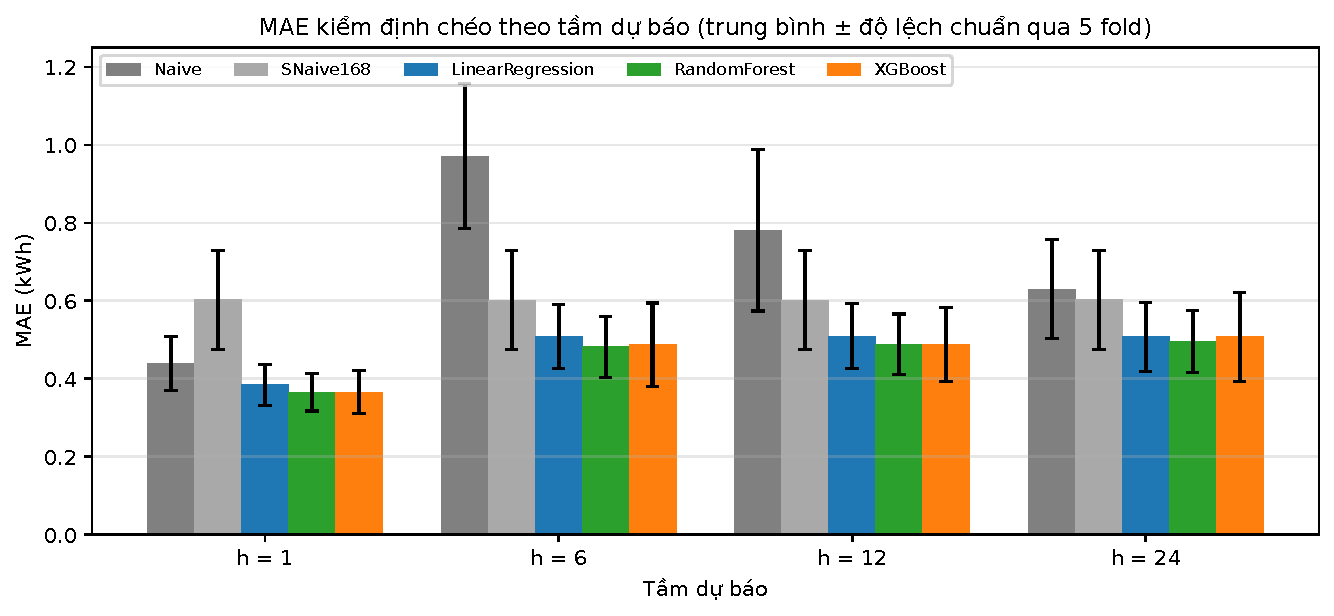
\includegraphics[width=0.92\textwidth]{figures/mae_theo_h.pdf}
    \caption{MAE kiểm định chéo theo tầm dự báo (trung bình $\pm$ độ lệch chuẩn qua 5 fold).}
    \label{fig:mae_h}
\end{figure}

\begin{table}[htbp]
\centering
\caption[So sánh mô hình học máy với mô hình cơ sở tốt nhất]{So sánh MAE trung bình của mô hình học máy với mô hình cơ sở tốt nhất ở từng tầm dự báo; cột cuối là số fold mô hình học máy có MAE thấp hơn.}
\label{tab:vs_baseline}
\small
\begin{tabular}{|c|c|l|c|c|c|}
\hline
\textbf{$h$} & \textbf{Cơ sở tốt nhất (MAE)} & \textbf{Mô hình} & \textbf{MAE} & \textbf{Giảm MAE (\%)} & \textbf{Số fold tốt hơn} \\
\hline
\multirow{3}{*}{1} & \multirow{3}{*}{Naive (0{,}440)} & LinearRegression & 0{,}384 & 12{,}7 & 5/5 \\
\cline{3-6}
 &  & RandomForest & 0{,}365 & 17{,}0 & 5/5 \\
\cline{3-6}
 &  & XGBoost & 0{,}366 & 16{,}9 & 5/5 \\
\hline
\multirow{3}{*}{6} & \multirow{3}{*}{SNaive168 (0{,}602)} & LinearRegression & 0{,}508 & 15{,}5 & 5/5 \\
\cline{3-6}
 &  & RandomForest & 0{,}482 & 20{,}0 & 5/5 \\
\cline{3-6}
 &  & XGBoost & 0{,}488 & 19{,}0 & 5/5 \\
\hline
\multirow{3}{*}{12} & \multirow{3}{*}{SNaive168 (0{,}602)} & LinearRegression & 0{,}509 & 15{,}4 & 5/5 \\
\cline{3-6}
 &  & RandomForest & 0{,}488 & 18{,}9 & 5/5 \\
\cline{3-6}
 &  & XGBoost & 0{,}488 & 18{,}8 & 5/5 \\
\hline
\multirow{3}{*}{24} & \multirow{3}{*}{SNaive168 (0{,}603)} & LinearRegression & 0{,}507 & 15{,}8 & 5/5 \\
\cline{3-6}
 &  & RandomForest & 0{,}495 & 17{,}8 & 5/5 \\
\cline{3-6}
 &  & XGBoost & 0{,}507 & 15{,}8 & 5/5 \\
\hline
\end{tabular}
\end{table}


Từ Bảng~\ref{tab:cv_summary}, Bảng~\ref{tab:vs_baseline} và Hình~\ref{fig:mae_h}:
\begin{enumerate}
    \item Cả ba mô hình học máy vượt mọi mô hình cơ sở ở mọi tầm dự báo và ở cả 5/5 fold, giảm MAE 12,7--20,0\% so với mô hình cơ sở tốt nhất. Mức mong muốn giảm ít nhất 10\% đặt ra ở Bảng~\ref{tab:objectives} đạt được với cả ba mô hình.
    \item Mô hình cơ sở tốt nhất thay đổi theo $h$. Naive tốt nhất ở $h = 1$ (MAE 0,440 kWh) nhưng kém nhất ở $h = 6$ (0,971 kWh, kém cả Mean), đúng như tự tương quan gần bằng 0 ở độ trễ 6. Từ $h = 6$, SNaive168 tốt nhất (khoảng 0,602 kWh).
    \item Random Forest có MAE thấp nhất hoặc ngang thấp nhất ở cả bốn tầm dự báo: 0,365 kWh ở $h = 1$ và 0,482--0,495 kWh ở $h \ge 6$. XGBoost gần như ngang Random Forest ở $h \le 12$ (chênh lệch không quá 0,006 kWh), nhưng ở $h = 24$ chỉ ngang Linear Regression (0,507 kWh) và có độ lệch chuẩn giữa các fold lớn nhất (0,115). Linear Regression kém hai mô hình cây 0,01--0,03 kWh.
    \item Các chênh lệch giữa ba mô hình học máy nhỏ hơn độ lệch chuẩn giữa các fold (0,05--0,12 kWh), nên với 5 fold chưa thể kết luận chắc chắn mô hình nào tốt nhất; chênh lệch giữa mô hình học máy và mô hình cơ sở thì rõ ràng và nhất quán ở mọi fold.
    \item MAPE của mô hình học máy vẫn cao (44--73\%) dù MAE dưới 0,51 kWh, do nhiều giờ có điện năng rất nhỏ. Điều này khớp với lý do không dùng MAPE làm chỉ số chính.
\end{enumerate}

\begin{figure}[htbp]
    \centering
    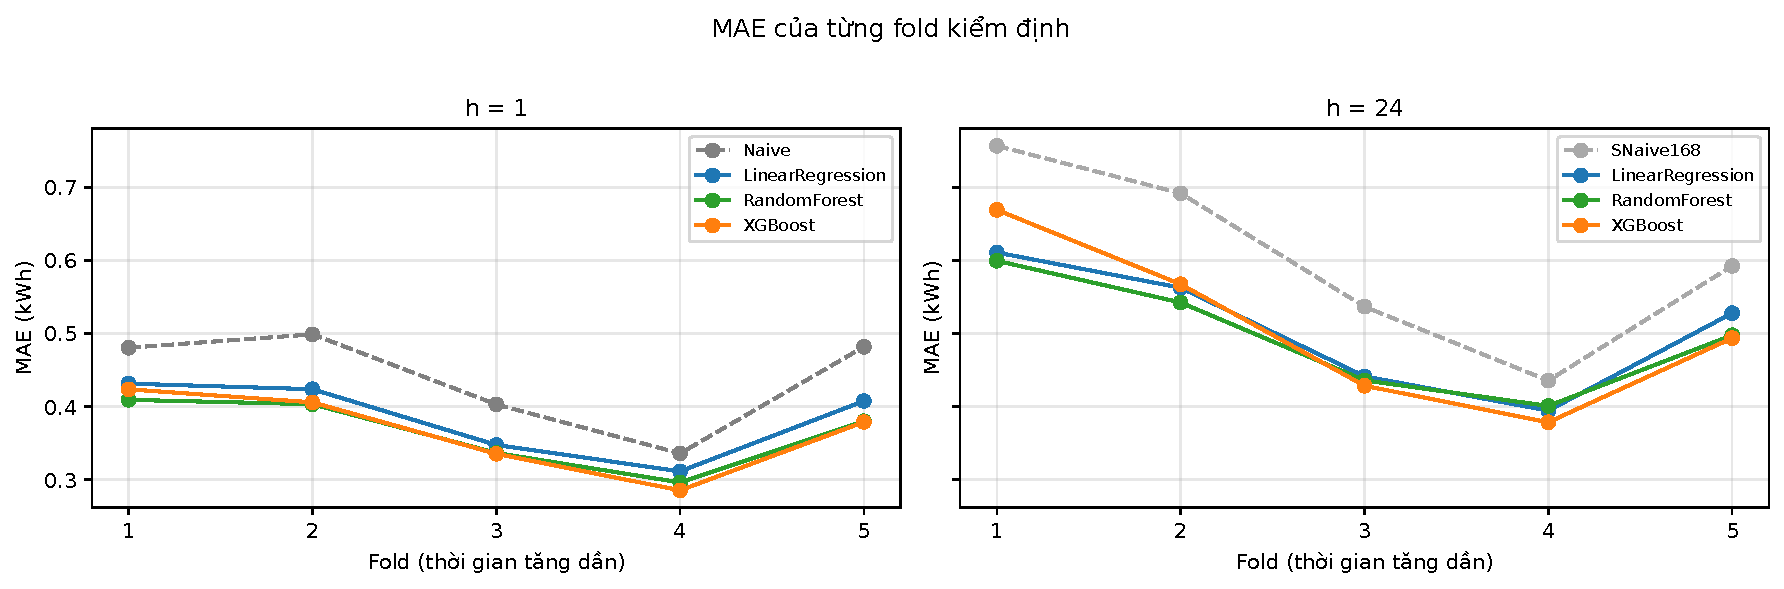
\includegraphics[width=\textwidth]{figures/mae_theo_fold.pdf}
    \caption{MAE của từng fold kiểm định với $h = 1$ (trái) và $h = 24$ (phải).}
    \label{fig:mae_fold}
\end{figure}

Hình~\ref{fig:mae_fold} cho thấy thứ hạng các mô hình gần như giữ nguyên qua các fold, còn mức sai số thay đổi theo mùa của phần kiểm định: fold 4 (07--10/2009, có tháng 8 tiêu thụ thấp) có MAE thấp nhất, fold 1 và 2 (mùa đông) cao nhất. Độ lệch chuẩn giữa các fold vì vậy chủ yếu phản ánh mức tiêu thụ của từng giai đoạn.

\section{Sai số trên phần huấn luyện và phần kiểm định}
\label{sec:train_val}

\begin{table}[htbp]
\centering
\caption[MAE trên phần huấn luyện và phần kiểm định]{MAE trung bình qua 5 fold trên phần huấn luyện (trong mẫu, ký hiệu HL) và phần kiểm định (KĐ), cùng tỷ số KĐ/HL.}
\label{tab:train_val}
\small
\begin{tabular}{|c|c|c|c|c|c|c|c|c|c|}
\hline
\multirow{2}{*}{\textbf{$h$}} & \multicolumn{3}{c|}{\textbf{Linear Regression}} & \multicolumn{3}{c|}{\textbf{Random Forest}} & \multicolumn{3}{c|}{\textbf{XGBoost}} \\
\cline{2-10}
 & HL & KĐ & KĐ/HL & HL & KĐ & KĐ/HL & HL & KĐ & KĐ/HL \\
\hline
1 & 0{,}409 & 0{,}384 & 0{,}94 & 0{,}241 & 0{,}365 & 1{,}51 & 0{,}265 & 0{,}366 & 1{,}38 \\ \hline
6 & 0{,}551 & 0{,}508 & 0{,}92 & 0{,}304 & 0{,}482 & 1{,}58 & 0{,}334 & 0{,}488 & 1{,}46 \\ \hline
12 & 0{,}551 & 0{,}509 & 0{,}93 & 0{,}308 & 0{,}488 & 1{,}59 & 0{,}338 & 0{,}488 & 1{,}45 \\ \hline
24 & 0{,}549 & 0{,}507 & 0{,}92 & 0{,}311 & 0{,}495 & 1{,}59 & 0{,}339 & 0{,}507 & 1{,}50 \\ \hline
\end{tabular}
\end{table}


\begin{figure}[htbp]
    \centering
    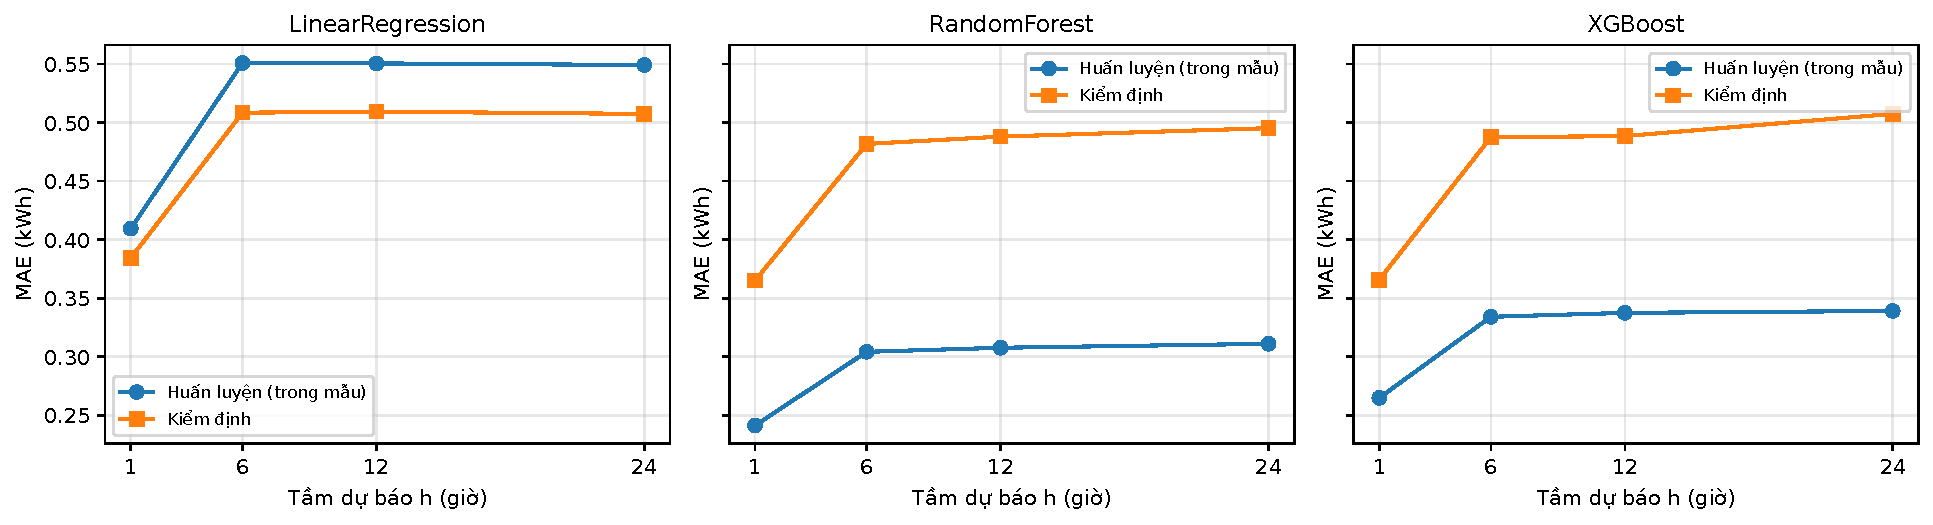
\includegraphics[width=\textwidth]{figures/train_val.pdf}
    \caption{MAE trên phần huấn luyện (trong mẫu) và phần kiểm định theo tầm dự báo.}
    \label{fig:train_val}
\end{figure}

Bảng~\ref{tab:train_val} và Hình~\ref{fig:train_val} cho thấy hai hành vi khác nhau:
\begin{itemize}
    \item Random Forest và XGBoost có MAE huấn luyện chỉ 0,24--0,34 kWh trong khi MAE kiểm định là 0,37--0,51 kWh (gấp 1,4--1,6 lần), và khoảng cách này xuất hiện ở mọi fold. Đây là dấu hiệu quá khớp. Tuy nhiên sai số huấn luyện ở đây là sai số trong mẫu, vốn luôn thấp với mô hình cây (mỗi lá của Random Forest chỉ cần 5 mẫu), nên cần kiểm chứng thêm bằng đường cong học tập và đường cong kiểm định ở giai đoạn tối ưu hóa.
    \item Linear Regression có sai số huấn luyện (0,41--0,55 kWh) xấp xỉ sai số kiểm định và cao hơn hẳn sai số huấn luyện của mô hình cây, tức mô hình chưa khớp: quan hệ tuyến tính không biểu diễn được tương tác giữa lịch và mức tiêu thụ gần đây. Sai số huấn luyện còn hơi lớn hơn sai số kiểm định vì phần huấn luyện chứa các mùa đông 2006--2008 tiêu thụ cao.
\end{itemize}

\section{Phân tích lỗi}
\label{sec:error_analysis}

Phân tích dùng dự báo của mọi mô hình trên phần kiểm định của cả 5 fold (từ 10/2008 đến 12/2009). Các hình dưới đây trình bày $h = 1$ và $h = 24$, hai đầu của dải tầm dự báo.

\begin{figure}[htbp]
    \centering
    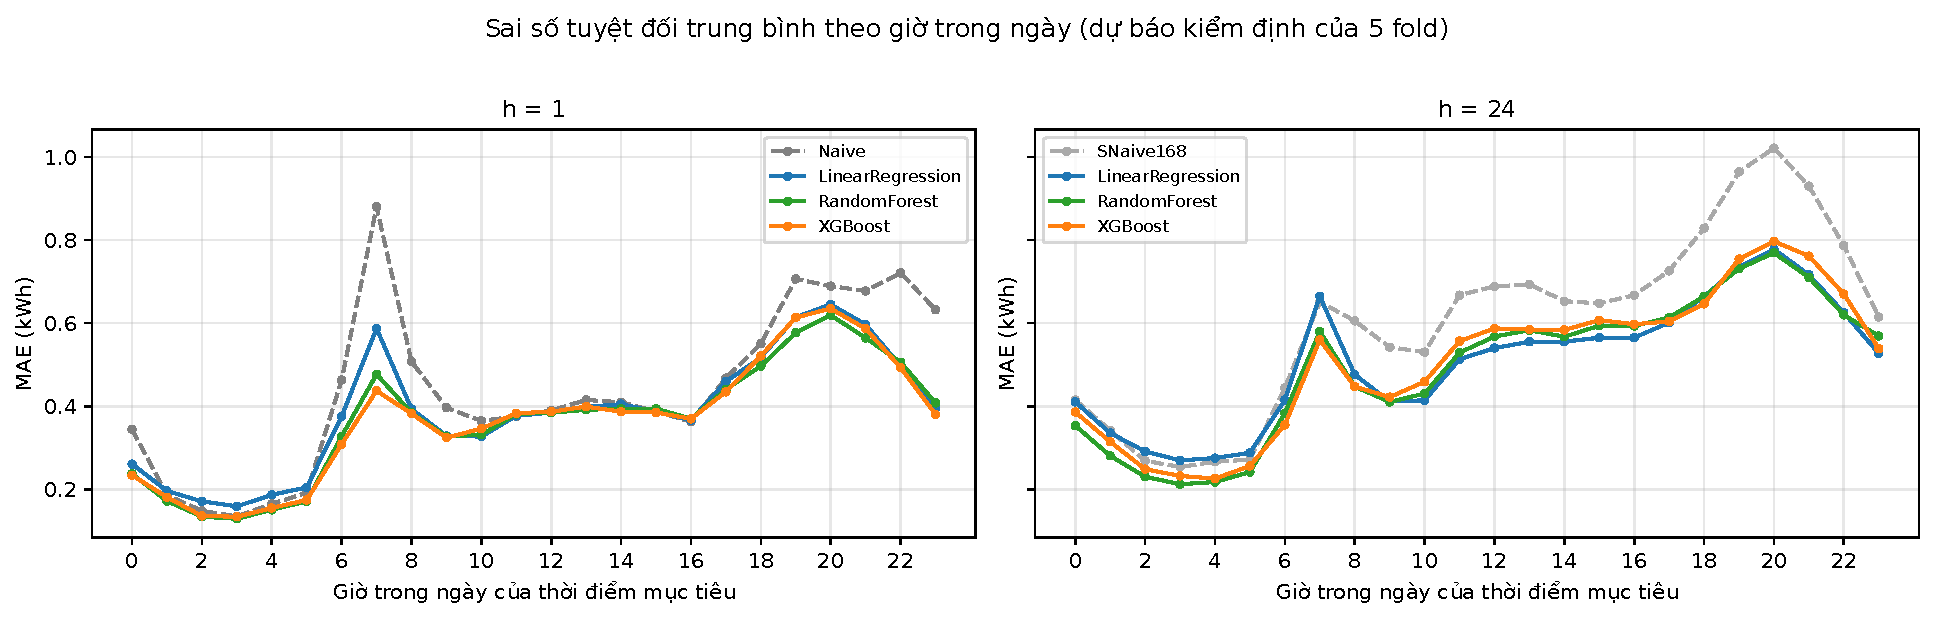
\includegraphics[width=\textwidth]{figures/mae_theo_gio.pdf}
    \caption{MAE theo giờ trong ngày của thời điểm mục tiêu.}
    \label{fig:mae_hour}
\end{figure}

\paragraph{Theo giờ trong ngày (Hình~\ref{fig:mae_hour}).} Sai số nhỏ nhất vào ban đêm (3 giờ: 0,13--0,16 kWh ở $h = 1$), khi hộ chỉ dùng tải nền. Đỉnh buổi tối 19--21 giờ là vùng khó nhất ở cả hai tầm dự báo: MAE của mô hình học máy là 0,56--0,65 kWh ở $h = 1$ và 0,71--0,80 kWh ở $h = 24$. Mô hình học máy cải thiện mạnh nhất ở đỉnh buổi sáng 7 giờ với $h = 1$ (Naive 0,88 kWh; Random Forest 0,48; XGBoost 0,44): Naive lặp lại giá trị 6 giờ còn thấp nên luôn trễ một bước khi tiêu thụ tăng, còn mô hình học máy biết từ đặc trưng giờ rằng 7 giờ thường tăng.

\begin{figure}[htbp]
    \centering
    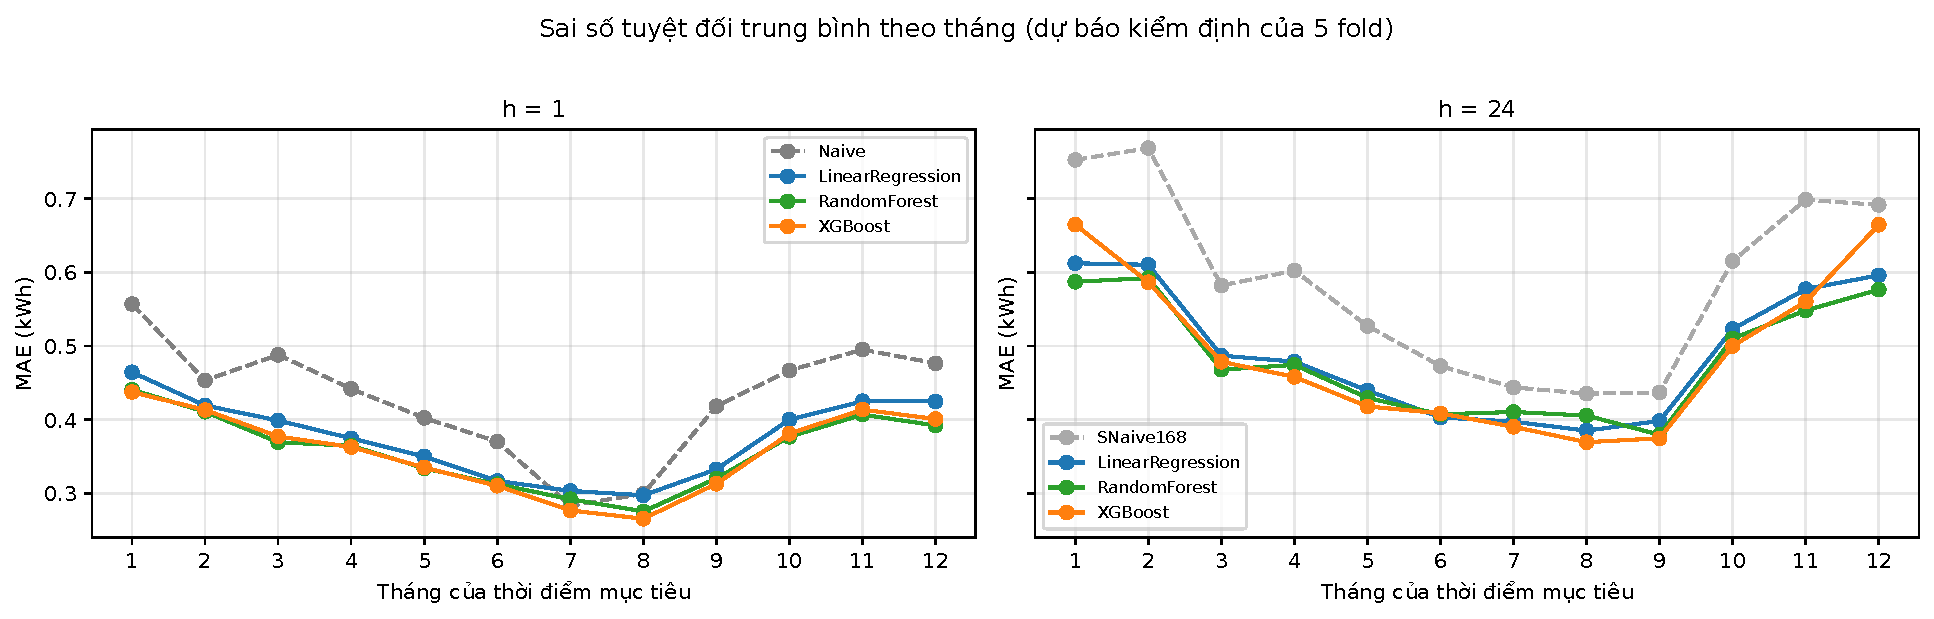
\includegraphics[width=\textwidth]{figures/mae_theo_thang.pdf}
    \caption{MAE theo tháng của thời điểm mục tiêu.}
    \label{fig:mae_month}
\end{figure}

\paragraph{Theo tháng (Hình~\ref{fig:mae_month}).} Sai số đi theo mức tiêu thụ: cao nhất vào mùa đông, thấp nhất vào tháng 7--8. Ở $h = 1$, tháng 7 là tháng duy nhất mô hình học máy không tốt hơn Naive rõ rệt (Naive 0,283; XGBoost 0,277; Linear Regression 0,303 kWh), vì khi tiêu thụ thấp và đều, giá trị giờ vừa qua đã là dự báo tốt. Ở $h = 24$, XGBoost có MAE tháng 1 và tháng 12 (cùng 0,665 kWh) cao hơn hẳn Random Forest (0,587 và 0,577), góp phần làm độ lệch chuẩn giữa các fold của XGBoost lớn hơn.

\begin{figure}[htbp]
    \centering
    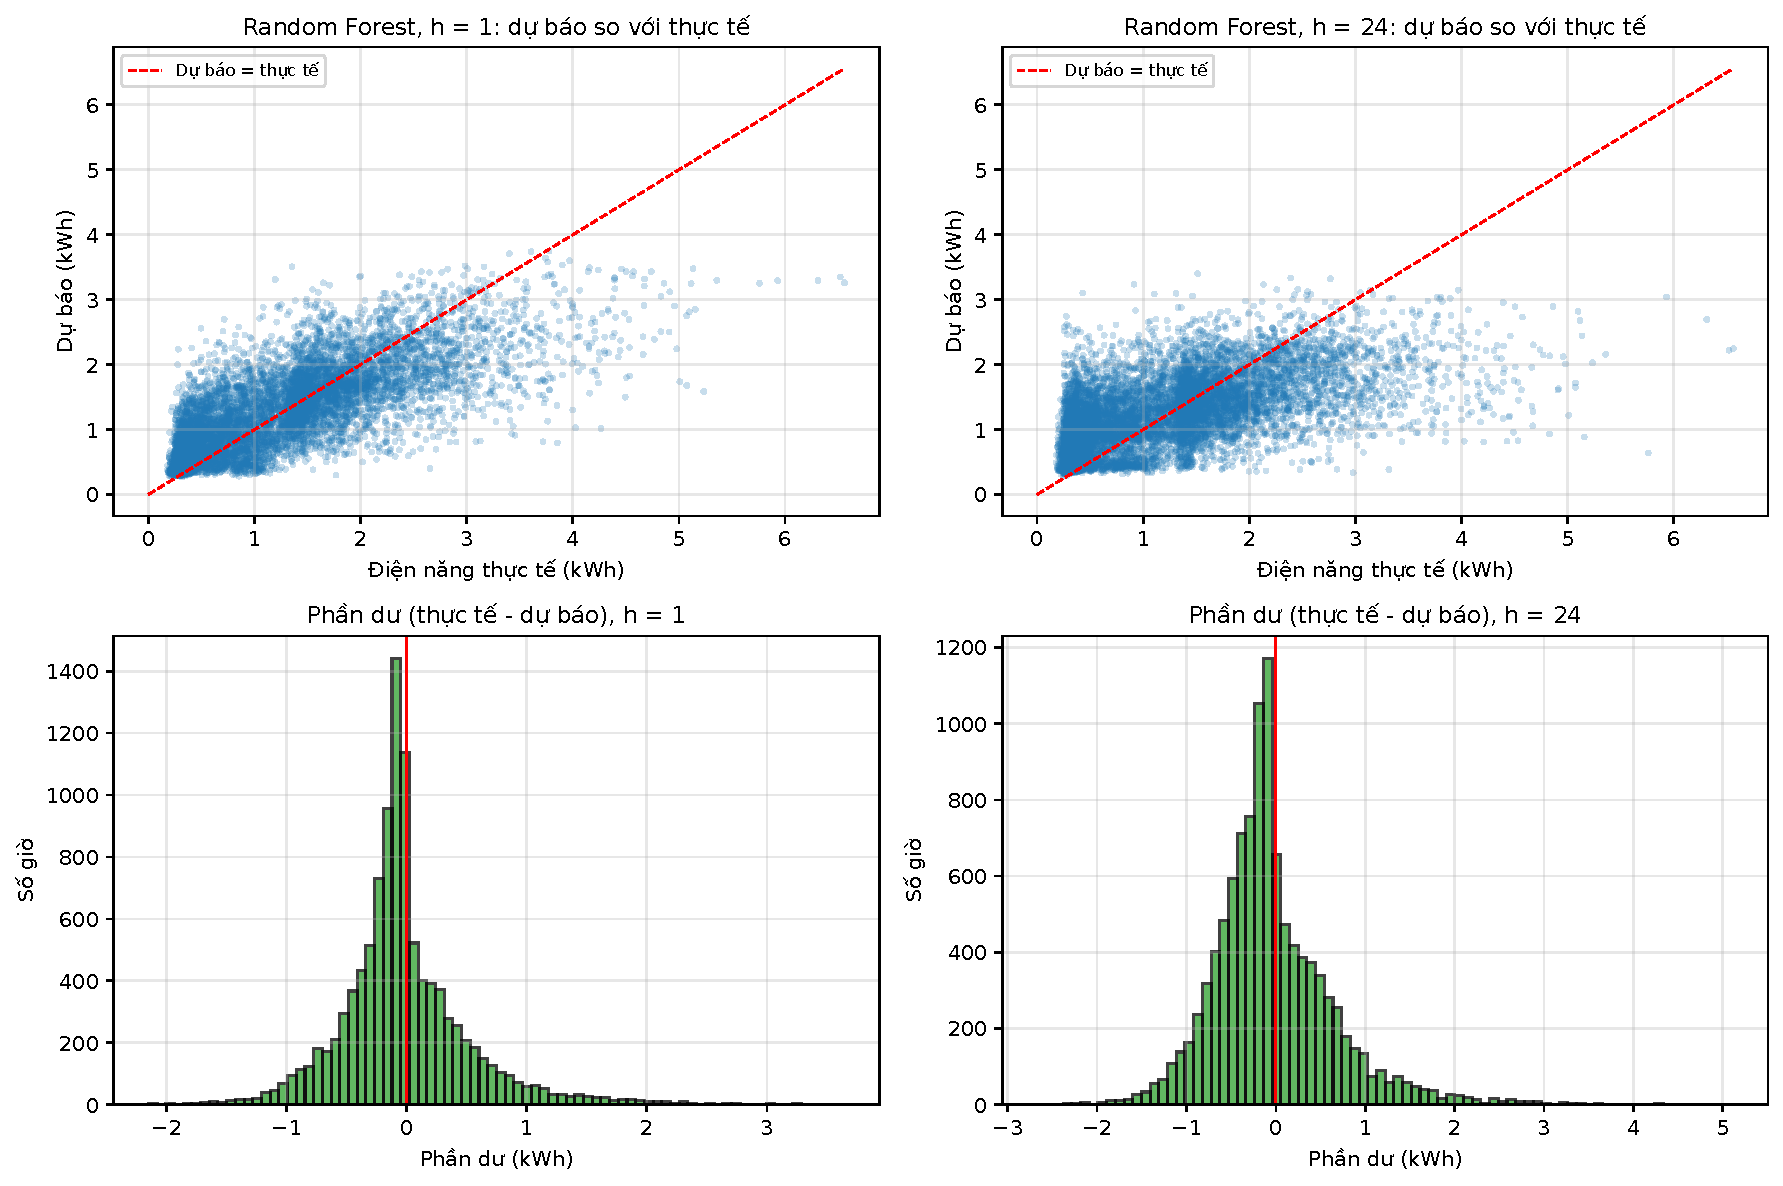
\includegraphics[width=0.95\textwidth]{figures/phan_du.pdf}
    \caption{Random Forest: dự báo so với thực tế (trên) và phân bố phần dư (dưới) với $h = 1$ và $h = 24$.}
    \label{fig:residuals}
\end{figure}

\begin{table}[htbp]
\centering
\caption[Mức độ tập trung của sai số]{Sai lệch trung bình (dự báo $-$ thực tế) ở nhóm giờ tiêu thụ cao nhất và thấp nhất, và tỷ trọng tổng sai số tuyệt đối do 10\% số giờ có sai số lớn nhất gây ra (dự báo kiểm định của 5 fold).}
\label{tab:error_conc}
\small
\begin{tabular}{|c|l|c|c|c|}
\hline
\textbf{$h$} & \textbf{Mô hình} & \textbf{5\% giờ cao nhất} & \textbf{10\% giờ thấp nhất} & \textbf{Tỷ trọng (\%)} \\
\hline
1 & LinearRegression & $-$1{,}112 & 0{,}214 & 33{,}2 \\ \hline
1 & RandomForest & $-$1{,}148 & 0{,}201 & 34{,}5 \\ \hline
1 & XGBoost & $-$1{,}061 & 0{,}189 & 34{,}4 \\ \hline
24 & LinearRegression & $-$1{,}626 & 0{,}425 & 30{,}6 \\ \hline
24 & RandomForest & $-$1{,}603 & 0{,}438 & 31{,}3 \\ \hline
24 & XGBoost & $-$1{,}436 & 0{,}440 & 31{,}6 \\ \hline
\end{tabular}
\end{table}


\paragraph{Phần dư và giờ đỉnh (Hình~\ref{fig:residuals}, Bảng~\ref{tab:error_conc}).} Các điểm ở vùng điện năng cao nằm dưới đường chéo: mô hình dự báo thấp các giờ đỉnh; ở $h = 24$ dự báo bị kéo về giá trị trung bình nhiều hơn. Phân bố phần dư lệch phải (skew 1,09 và 1,13): phần lớn giờ có phần dư âm nhỏ (dự báo hơi cao ở giờ tải nền, trung vị $-0{,}074$ và $-0{,}128$ kWh), xen với một số ít giờ có phần dư dương rất lớn. Ở 5\% giờ tiêu thụ cao nhất (từ 2,81 kWh), mô hình dự báo thấp trung bình 1,06--1,15 kWh với $h = 1$ và 1,44--1,63 kWh với $h = 24$; 10\% số giờ có sai số lớn nhất chiếm 30,6--34,5\% tổng sai số tuyệt đối. Trung bình phần dư gần 0 ($-0{,}02$ và $-0{,}04$ kWh), nên mô hình gần như không lệch hệ thống; sai số chủ yếu đến từ việc không đoán được thời điểm và độ lớn của đỉnh, vốn phụ thuộc vào hành vi khó đoán như bật nhiều thiết bị cùng lúc.

\begin{figure}[htbp]
    \centering
    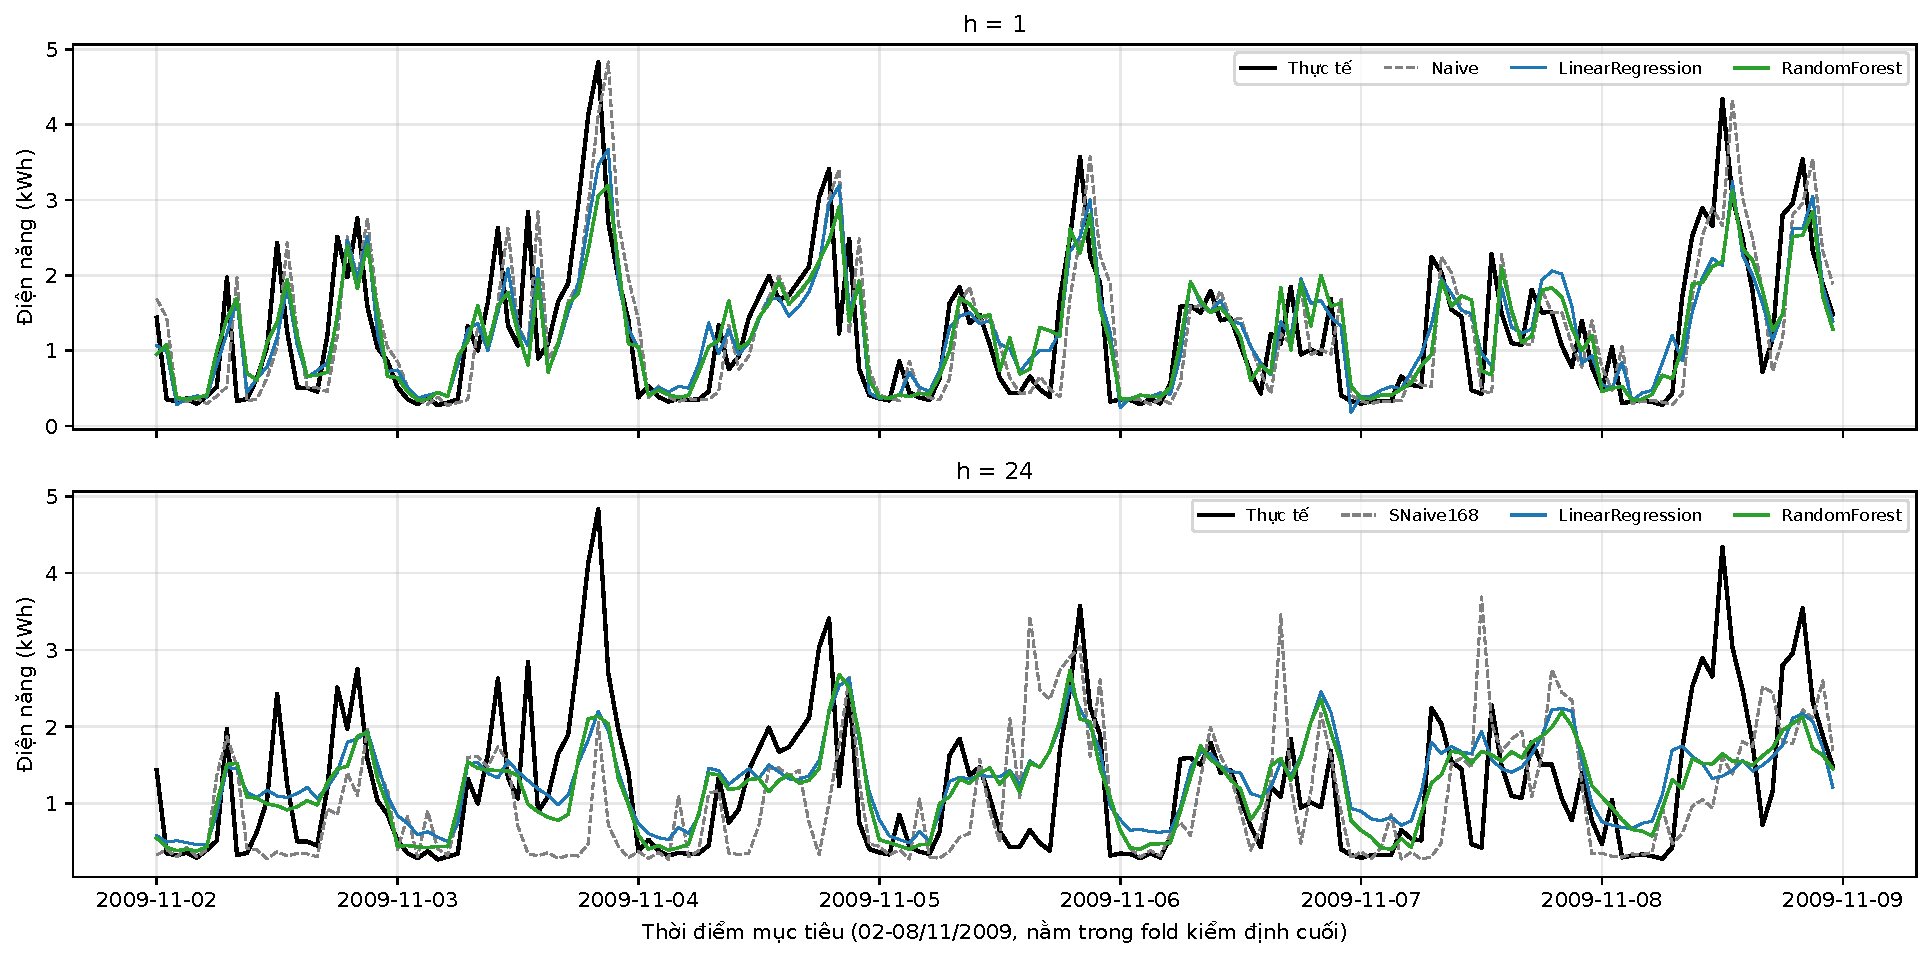
\includegraphics[width=\textwidth]{figures/tuan_vi_du.pdf}
    \caption{Dự báo và thực tế trong tuần 02--08/11/2009 (thuộc fold kiểm định cuối).}
    \label{fig:week}
\end{figure}

\paragraph{Ví dụ một tuần (Hình~\ref{fig:week}).} Với $h = 1$, các mô hình bám sát đường thực tế nhưng trễ khoảng một giờ ở các lần tăng đột ngột, và không đạt tới đỉnh 4,8 kWh tối 03/11 (Random Forest khoảng 3,2 kWh). Với $h = 24$, dự báo mượt hơn hẳn: mô hình tái hiện được nhịp tăng buổi tối hằng ngày nhưng gần như bỏ qua các đỉnh riêng lẻ, còn SNaive168 sao chép nguyên tuần trước nên có những đỉnh không xảy ra trong tuần này.

\section{Đặc trưng ảnh hưởng đến dự báo}
\label{sec:importance}

\begin{figure}[htbp]
    \centering
    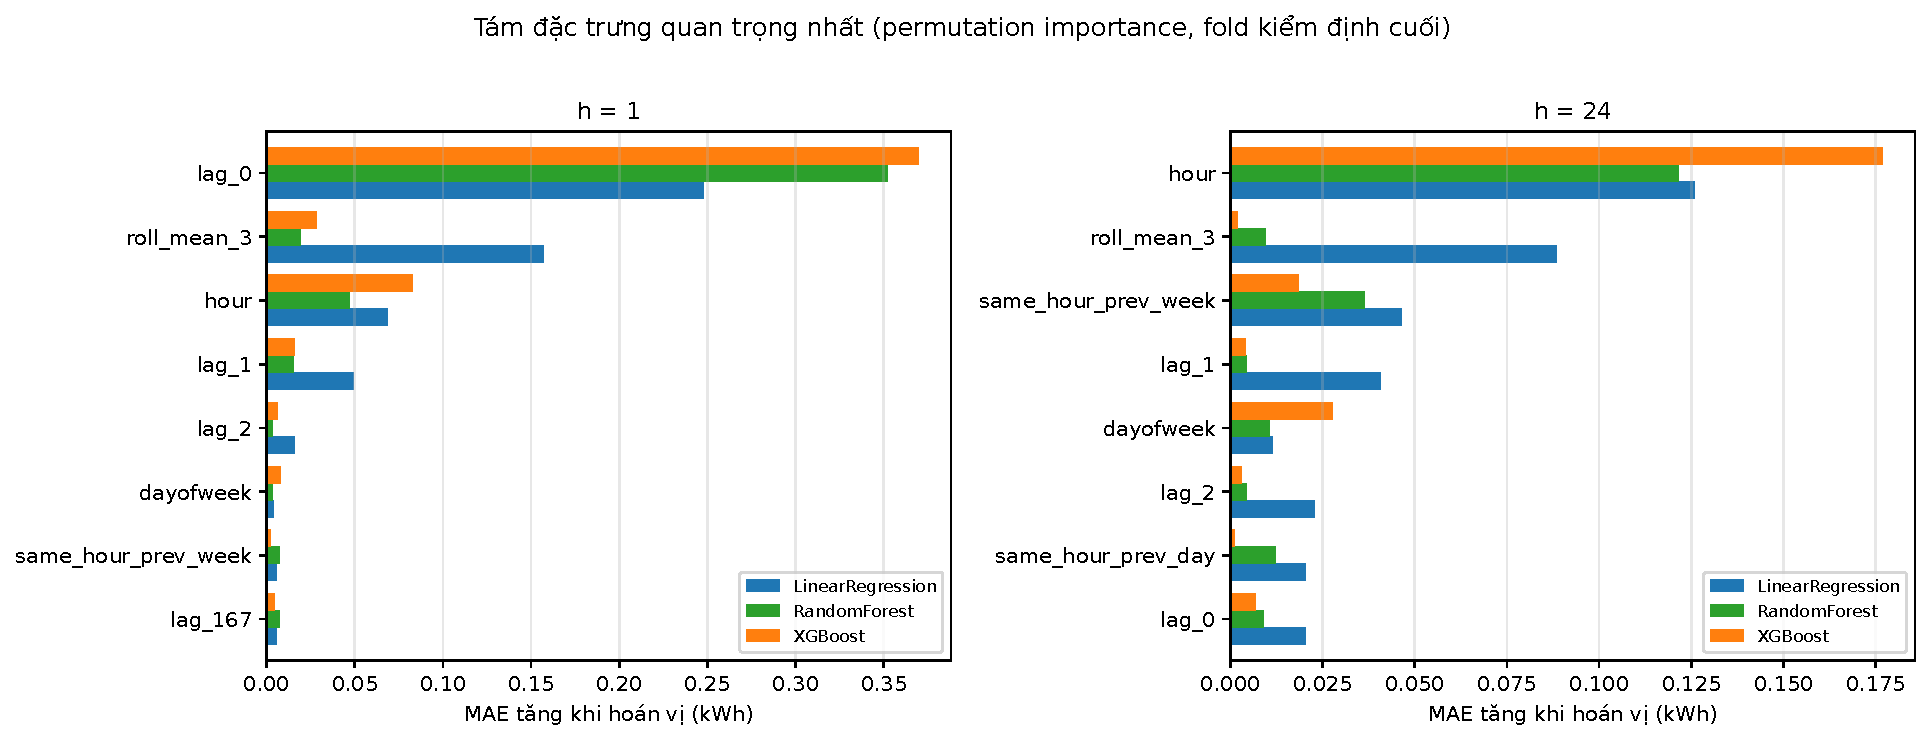
\includegraphics[width=\textwidth]{figures/tam_quan_trong.pdf}
    \caption{Tám đặc trưng quan trọng nhất theo permutation importance (MAE tăng khi hoán vị, phần kiểm định của fold cuối, 5 lần lặp).}
    \label{fig:importance}
\end{figure}

Hình~\ref{fig:importance} cho thấy cơ chế dự báo thay đổi theo tầm dự báo:
\begin{itemize}
    \item $h = 1$: thông tin về vài giờ vừa qua áp đảo. Với hai mô hình cây, hoán vị $y_t$ (điện năng giờ vừa qua) làm MAE tăng 0,35--0,37 kWh; Linear Regression chia tầm quan trọng này giữa $y_t$ (0,25) và trung bình 3 giờ gần nhất (0,16), vì trung bình này chứa chính $y_t$. Tiếp theo là giờ trong ngày (0,05--0,08).
    \item $h = 24$: giờ trong ngày trở thành quan trọng nhất (0,12--0,18 kWh), tiếp theo là giá trị cùng giờ tuần trước $y_{t+h-168}$ (0,02--0,05) và ngày trong tuần. Mô hình chủ yếu học hồ sơ tiêu thụ theo giờ và thứ, cộng với giá trị cùng giờ tuần trước.
\end{itemize}
Các đặc trưng tương quan với nhau chia sẻ tầm quan trọng; ví dụ ở $h = 24$, $y_t$ và giá trị cùng giờ ngày trước $y_{t+h-24}$ là cùng một giá trị. Kết quả này khớp với nhận xét ở Mục~\ref{sec:correlation}: tự tương quan bậc 1 cao quyết định dự báo ngắn hạn, còn chu kỳ ngày và tuần quyết định dự báo xa hơn.

\section{Thảo luận}
\label{sec:discussion}

\paragraph{Vì sao mô hình cây tốt hơn Linear Regression.} Điện năng phụ thuộc vào tương tác giữa giờ, thứ, tháng và mức tiêu thụ gần đây (ví dụ cùng là 20 giờ nhưng mùa đông và mùa hè khác nhau). Linear Regression chỉ cộng các tác động riêng lẻ nên chưa khớp; mô hình cây tự chia dữ liệu theo các tổ hợp này. Lợi thế của mô hình cây rõ nhất ở đỉnh buổi sáng và buổi tối, nơi tương tác giữa giờ và mức tiêu thụ trước đó mạnh nhất.

\paragraph{Vì sao lợi thế so với mô hình cơ sở gần như không đổi theo $h$.} Mức giảm MAE so với mô hình cơ sở tốt nhất là 17--20\% với Random Forest ở mọi $h$. Ở $h = 1$, mô hình cải thiện so với Naive nhờ biết giờ trong ngày; ở $h \ge 6$, mô hình cải thiện so với SNaive168 nhờ kết hợp nhiều chu kỳ thay vì sao chép một tuần duy nhất.

\paragraph{Hạn chế ở giai đoạn này.} (i) Siêu tham số chưa được tối ưu và mô hình cây có dấu hiệu quá khớp chưa được kiểm chứng đầy đủ. (ii) Mô hình dự báo thấp có hệ thống các giờ đỉnh. (iii) Bộ đặc trưng chưa có thông tin ngày lễ và giá trị trễ của các nhóm công tơ phụ. (iv) Kết quả mới là kiểm định chéo trên tập huấn luyện; tập kiểm tra năm 2010 sẽ chỉ được dùng một lần cho mô hình cuối ở giai đoạn tối ưu hóa, để ước lượng sai số trên dữ liệu mới không bị ảnh hưởng bởi các lựa chọn của nhóm.

\unnumberedchapter{KẾT LUẬN}
\label{chap:conclusion}

\plainheading{1. Kết quả đạt được}
Đến giai đoạn hiện tại, nhóm đã hoàn thành hai phần đầu của quy trình học máy cho bài toán dự báo điện năng tiêu thụ theo giờ của hộ gia đình:
\begin{itemize}
    \item \textbf{Bài toán và dữ liệu:} phát biểu bài toán hồi quy với đơn vị mẫu, đầu vào, đầu ra và tầm dự báo cụ thể; chọn MAE làm chỉ số chính; lập từ điển dữ liệu; khảo sát phân bố, tương quan, tự tương quan và tính mùa vụ theo giờ, ngày, tháng.
    \item \textbf{Chất lượng và chuẩn bị dữ liệu:} định lượng các vấn đề chất lượng, nổi bật là 25.979 phút thiếu tập trung thành 71 khối; tổng hợp nhãn theo giờ không nội suy; chia dữ liệu theo thời điểm mục tiêu; kiểm định chéo \code{TimeSeriesSplit} có khoảng đệm; đường ống tiền xử lý chỉ học trên tập huấn luyện.
    \item \textbf{Mô hình:} trên kiểm định chéo 5 fold, cả ba mô hình Linear Regression, Random Forest và XGBoost đều vượt mọi mô hình cơ sở ở cả bốn tầm dự báo và ở mọi fold, giảm MAE 12,7--20,0\% so với mô hình cơ sở tốt nhất. Random Forest có MAE thấp nhất (0,365 kWh ở $h = 1$; 0,482--0,495 kWh ở $h \ge 6$). Quy trình chạy lại được từ đầu trong môi trường mới và cho kết quả trùng khớp.
\end{itemize}

\plainheading{2. Hạn chế}
\begin{itemize}
    \item Dữ liệu của một hộ duy nhất, không có thông tin thời tiết; các giải thích về hành vi sinh hoạt (kỳ nghỉ tháng 8, sưởi mùa đông) mới là giả thuyết.
    \item Mô hình dự báo thấp các giờ đỉnh và sai số tập trung ở khung 19--21 giờ; mô hình cây có dấu hiệu quá khớp chưa được kiểm chứng đầy đủ.
    \item Siêu tham số chưa được tối ưu và mô hình chưa được đánh giá trên tập kiểm tra.
\end{itemize}

\plainheading{3. Hướng phát triển}
\begin{itemize}
    \item Kiểm chứng quá khớp bằng đường cong học tập và đường cong kiểm định; tối ưu siêu tham số bằng tìm kiếm trên cùng các fold kiểm định chéo.
    \item Cải tiến đặc trưng (ngày lễ, giá trị trễ của các nhóm công tơ phụ) và thử phương pháp tổ hợp mô hình, so sánh trước -- sau trên cùng điều kiện.
    \item Đánh giá mô hình cuối một lần trên tập kiểm tra năm 2010 và so sánh với kết quả kiểm định chéo.
\end{itemize}


% ------------------------------------------------------------------------------
% 4. TÀI LIỆU THAM KHẢO
% ------------------------------------------------------------------------------
\clearpage
\printbibliography[heading=bibintoc,title={TÀI LIỆU THAM KHẢO}]

% ------------------------------------------------------------------------------
% 5. PHỤ LỤC
% ------------------------------------------------------------------------------
\clearpage
\appendix
\addtocontents{toc}{\protect\renewcommand*{\protect\chaptername}{PHỤ LỤC}}
\chapter{MÃ NGUỒN VÀ TÁI LẬP}
\label{app:code}

\section{Tổ chức mã nguồn}
Mã nguồn được lưu tại kho \url{https://github.com/HoanBuCon/machine-learning} và tổ chức như sau:
\begin{itemize}
    \item \code{notebooks/01_eda.ipynb}: tải và đọc dữ liệu, khảo sát, chất lượng dữ liệu, tạo bảng điện năng theo giờ.
    \item \code{notebooks/02_chuan_bi_du_lieu.ipynb}: bảng có giám sát, chia theo thời gian, kiểm định chéo, đường ống tiền xử lý.
    \item \code{notebooks/03_huan_luyen_danh_gia.ipynb}: mô hình cơ sở, mô hình học máy, kiểm định chéo, phân tích lỗi.
    \item \code{src/features.py}, \code{src/models.py}, \code{src/evaluation.py}: mã dùng chung cho đặc trưng, mô hình và đánh giá.
    \item \code{ket_qua/}: bảng kết quả do notebook 03 ghi ra; \code{bao_cao/}: báo cáo này, kèm script xuất hình và sinh bảng.
\end{itemize}

\section{Hướng dẫn tái lập}
Với Python 3.11, trong thư mục gốc của kho mã:
\begin{lstlisting}[language=bash]
python -m venv .venv
.venv\Scripts\activate
pip install -r requirements.txt
cd notebooks
jupyter nbconvert --to notebook --execute --inplace 01_eda.ipynb 02_chuan_bi_du_lieu.ipynb 03_huan_luyen_danh_gia.ipynb
\end{lstlisting}
Notebook 01 tự tải dữ liệu từ UCI (khoảng 20 MB) nếu chưa có. Mọi mô hình dùng \code{random_state = 42}.

\chapter{KHAI BÁO SỬ DỤNG CÔNG CỤ TRÍ TUỆ NHÂN TẠO}
\label{app:ai}

\begingroup
\setstretch{1.15}
\noindent
\begin{tabularx}{\textwidth}{|>{\raggedright\arraybackslash}p{2.8cm}|>{\raggedright\arraybackslash}X|>{\raggedright\arraybackslash}X|}
\hline
\textbf{Công cụ} & \textbf{Phạm vi sử dụng} & \textbf{Phần do nhóm thực hiện và kiểm chứng} \\ \hline
Claude Code (Anthropic) và Codex (OpenAI) &
- Hướng dẫn, định hướng các bước thực hiện dự án.\newline
- Rà soát mã nguồn và nhận xét trong notebook; đề xuất và sinh một số đoạn mã.\newline
- Tính lại độc lập để kiểm tra các con số trong nhận xét.\newline
- Tra cứu, xác minh tài liệu tham khảo.\newline
- Hỗ trợ soạn bản nháp báo cáo LaTeX. &
- Chọn đề tài, bộ dữ liệu; quyết định hướng tiếp cận và cách xử lý dữ liệu.\newline
- Viết mã notebook với sự hỗ trợ của công cụ; đọc hiểu, chỉnh sửa và quyết định giữ hay bỏ từng đoạn.\newline
- Chạy lại toàn bộ notebook, đối chiếu số liệu trong báo cáo với kết quả chạy.\newline
- Chỉnh sửa nội dung; chịu trách nhiệm về toàn bộ báo cáo và giải thích được mọi phần khi vấn đáp. \\ \hline
\end{tabularx}
\endgroup


\end{document}
